\documentclass[a4paper,12pt]{extarticle} % На предупрежденгие насрать, все норм компиилирутся и славно
% Глобальные поля
\usepackage[left=30mm, top=20mm, right=15mm, bottom=20mm,nohead, includefoot,footskip=35pt]{geometry}

% Язык, кодировка, шрифт
\usepackage[utf8]{inputenc}
\usepackage[T1]{fontenc}
\usepackage[english]{babel}
%\renewcommand{\rmdefault}{Tempora-TLF}
\usepackage{mathptmx}

\usepackage[
    backend=biber,
    style=gost-authoryear,
    movenames=false, % Если авторов больше 4 кеакого-то хрена меняло на название работы
    otherlangs=true
]{biblatex}
\addbibresource{bibliography.bib}
\usepackage{csquotes}

% Межстрочный интервал = 1.5pt
\usepackage{setspace}
\onehalfspacing

% Абзацный отступ = 1.25см
\usepackage{indentfirst}
\setlength\parindent{12.5mm}

% Пакет для содержания
\usepackage{tocloft}

% Команда для специальных разделов (введение, обзор литературы, etc)
% Не нумеруются в содержании, по уровню вложенности:
\newcommand{\specialsection}[1]{
    \phantomsection
    \bigskip\smallskip\hspace{-13.8mm}
    \normalfont\fontsize{12}{12}\textbf{#1}
    \par\bigskip\normalfont\normalsize
    \addcontentsline{toc}{section}{#1}
}

% Размеры заголовков разделов и подразделов
\usepackage{titlesec}
% Раздел: 12pt, добавляем слово "CHAPTER"
\titleformat{\section}
{\fontsize{12}{12}\bfseries}{
\hspace{-1.5mm}CHAPTER \thesection. \hskip-1em}{1em}{}
% Подраздел: 12pt
\titleformat{\subsection}
{\fontsize{12}{12}\bfseries}{\hspace{-0.2mm}\thesubsection}{1em}{}

% Содержание
\renewcommand{\cfttoctitlefont}{\centering\normalsize\bfseries}
\renewcommand{\cftaftertoctitle}{\hfill}

% Слово "Глава" в содержании
\renewcommand{\cftsecpresnum}{CHAPTER\space}
\newlength\mylength
\settowidth\mylength{\cftsecpresnum}
\addtolength\cftsecnumwidth{\mylength}
% Строки с точками
\renewcommand{\cftsecleader}{\cftdotfill{\cftdotsep}}
% Точки после цифр в в содержании
\renewcommand{\cftsecaftersnum}{.}
\renewcommand{\cftsubsecaftersnum}{.}
% Подровнять subsection под точку главы
% (если глав будет больше десяти, будет чуть хуже)
\setlength{\cftsubsecindent}{2.68em}
% Интервал глав
\setlength{\cftbeforesecskip}{4pt}

\renewcommand{\cftsecpagefont}{\normalfont}

% Шрифт подписи (caption) = 12pt
% (Повезло, что small как раз равен 12pt)
\usepackage[font=small,labelfont=bf]{caption}

% Пакет, который позволяет собирать один документ TeX из нескольких
\usepackage{import}

% Пакет, реализующий гиперссылки. Никакого расскрашивания
\usepackage[colorlinks=false,unicode=true]{hyperref}

\newcommand{\ITEM}{\vspace{-0.2cm}\item}
\newcommand{\MList}[1]{\par\begin{itemize}#1\end{itemize}}
\newcommand{\NList}[1]{\par\begin{enumerate}#1\end{enumerate}}


% Задаем отступ у списков равным обычному абзацному отступу (\parindent)
\usepackage{enumitem}
\setlist[itemize]{leftmargin=\dimexpr\parindent\relax}
\setlist[enumerate]{leftmargin=\dimexpr\parindent\relax}

% Нумерация только тех формул, на которые в тексте присутствует ссылка
% \usepackage{autonum}
% Правка нумерации формул: числа справа в скобках
\renewcommand{\theequation}{\arabic{equation}}

% Список литературы
% \makeatletter
% \renewenvironment{thebibliography}[1]
%     {%
%       \bigskip
%       {\noindent\normalfont\bfseries References\par}%
%       \addcontentsline{toc}{section}{References}%
%       \smallskip
%       \list{\@biblabel{\@arabic\c@enumiv}}%
%            {%
%              \settowidth\labelwidth{\@biblabel{#1}}%
%              \leftmargin\labelwidth
%              \advance\leftmargin\labelsep
%              \@openbib@code
%              \usecounter{enumiv}%
%              \let\p@enumiv\@empty
%              \renewcommand\theenumiv{\@arabic\c@enumiv}%
%            }%
%       \sloppy
%       \clubpenalty4000
%       \@clubpenalty \clubpenalty
%       \widowpenalty4000%
%       \sfcode`\.\@m%
%     }%
%     {%
%       \def\@noitemerr
%         {\@latex@warning{Empty `thebibliography' environment}}%
%       \endlist%
%     }
% \makeatother


% Пакеты по желанию (самые распространенные)
% Хитрые мат. символы
\usepackage{euscript}
% Таблицы
\usepackage{multirow}
\usepackage{longtable}
\usepackage{makecell}
% Картинки (можно встявлять даже pdf)
\usepackage[pdftex]{graphicx}

\usepackage{amsthm,amssymb,amsmath}
\usepackage{textcomp}

% Для коректной работы H в фигурах и ссылок на фигуры
\usepackage{float}

\usepackage{hyperref}

\newcommand{\argmax}{\operatornamewithlimits{argmax}}
\newcommand{\argmin}{\operatornamewithlimits{argmin}}
\DeclareMathOperator{\col}{col}
\usepackage{pdfpages}
\begin{document}
    % Оглавление
    %% Титульный лист диплома СПбГУ
% Временное удаление foot на titlepage
\newgeometry{left=30mm, top=20mm, right=15mm, bottom=20mm, nohead, nofoot}
\begin{titlepage}
\begin{center}

\textbf{Saint Petersburg}
\textbf{State University}

\vspace{35mm}

\textbf{\textit{\large Tomin Denis Valerievich}} \\[8mm]
% Название
\textbf{\large Bachelor Diploma Thesis}\\[3mm]
\textbf{\textit{\large Understanding the Aspect Structure of Financial Publications Using Deep Neural Networks}}

\vspace{20mm}
Level of education: Bachelor's degree\\
Direction 01.03.02 “Applied Mathematics and Informatics”\\
Basic educational program CB.5005.2015
«Management»\\
Graduated School of Management\\[25mm]


% Научный руководитель, рецензент
\begin{flushright}
\begin{minipage}[t]{0.65\textwidth}
{Supervisor:} \\
Professor, Research Center for Market Efficiency and Applied Finance, \\ Dr. Darko Vuković

\vspace{10mm}

{Peer reviewer:} \\
Senior Lecturer, Department of Finance and Accounting, \\ Vitaly Leonidovich Okulov
\end{minipage}
\end{flushright}

\vfill

{Saint Petersburg}
\par{\the\year{}}
\end{center}
\end{titlepage}
% Возвращаем настройки geometry обратно (то, что объявлено в преамбуле)
\restoregeometry
% Добавляем 1 к счетчику страниц ПОСЛЕ titlepage, чтобы исключить
% влияние titlepage environment
\addtocounter{page}{1}
    %\pagebreak

    % Заявлениее о самостоятльности
    %\input{}
    %\pagebreak
    
\includepdf[pages=-,             % все страницы файла
            noautoscale=true,    % не менять масштаб
            offset=0mm 0mm,      % поправка позиционирования
            pagecommand={\thispagestyle{empty}}
           ]{struct/start-1.5.pdf}

    % Оглавленине
    \tableofcontents{}
    \pagebreak

    \specialsection{Введение}
    \label{sec:introduction}
    In recent years, the use of data analytics and artificial intelligence, specifically machine learning (ML) and deep learning (DL),
to make investment decisions has become an integral part of many companies' and funds' strategies. However, today's financial
markets are characterized by high volatility and high speed of information dissemination, which creates significant challenges
for analyzing its impact on stock prices.

Events such as news releases, regulatory changes and analysts' reviews can have both immediate and cumulative effects
on market performance. However, traditional approaches to analyzing data often ignore the dynamics of these influences,
resulting in poor forecast accuracy and, consequently, ineffective investment strategies.

To compete in a rapidly changing financial environment, companies need to continuously optimize their approaches to data analysis.
This requires the development of tools that can not only account for the dynamic nature of information, but also provide forecasts
based on an in-depth analysis of events and their cumulative effect. This paper responds to these challenges by proposing
a methodology and a technological solution for more accurate stock price forecasting based on deep neural networks,
namely large language models (LLM).

Classical ML algorithms have demonstrated their effectiveness in financial forecasting in numerous studies.
However, DL and natural language processing (NLP) architectures have fundamentally shifted the paradigm following
the emergence of the Transformer architecture in 2017 \parencite{vaswani2017attention}. Since then, LLMs
have gained wide acceptance and proven their applicability across various applied tasks, including asset price forecasting
\parencite{Jiang2023, Halder2022, Kim2023}.

Contemporary research demonstrates the high efficacy of LLMs in addressing a range of tasks related to asset evaluation and forecasting.
Nevertheless, unresolved issues remain regarding the integration of LLMs with classic quantitative models, the scarcity of open-source
solutions for the financial domain, and the limitations of current models in processing long textual sequences (see Section 1.3.1).
In December 2024, a new state-of-the-art (SoTA) model, ModernBERT, was introduced, capable of processing texts that are 16 times longer
than those handled by previous architectures \parencite{Warner2024ModernBERT, devlin2019BERT}. This model extends analytical capabilities
from isolated headlines or posts to full news articles, press releases, interview transcripts, and analytical reviews. Nonetheless,
processing comprehensive financial reports (e.g., 10-Q, 10-K) remains a challenging task (see Section 2.1.4). Moreover,
focusing on full articles helps to mitigate issues related to clickbait and insufficient context.

Pre-trained language models on general text corpora do not always effectively address financial forecasting tasks \parencite{Jiang2023}.
This is due to the unique nature of financial information, characterized by specialized terminology and jargon, which complicates
the application of general-purpose models. Consequently, there is a need to adapt baseline LLMs for the financial domain.

From a management perspective, when making investment decisions in volatile markets, it is crucial to promptly analyze the cumulative
impact of various events (news, regulatory changes, analyses, etc.) on asset dynamics. Experts are unable to process such an immense
volume of information within extremely short time frames. Conversely, the absence of a comprehensive analysis tool leads to delayed
or inaccurate decisions, reducing the effectiveness of investment strategies and increasing the risk of missing lucrative opportunities.

The development of such a tool is complex and demanding, and it can be conceptually divided into the following stages:
\begin{enumerate}
    \item Development of an effective architecture for LLMs.
    \item Adaptation of the model to the specifics of the financial domain.
    \item Fine-tuning of the model to address particular tasks.
    \item Integration of the model into a system operating with both quantitative and qualitative data, encompassing training, testing,
    and deployment processes.
\end{enumerate}

Since the basic architecture of ModernBERT has already been established, the present study focuses on its domain adaptation.
Among the available adaptation methods --- fine-tuning, complete retraining, and domain-adaptive pretraining --- the latter is emphasized
in this work (see Section 1.3.2), as it minimizes time, computational, and financial costs.

Within the scope of this research, hierarchical aspect-based analysis of financial publications (see Section 3.2) is considered
an effective task for financial forecasting. The object of the study is investment strategies based on the use of artificial intelligence,
while the subject is the integration of language models into asset price forecasting processes. The goal of this work is to develop
a practice-oriented toolkit for dynamic multimodal forecasting using aspect-based sentiment analysis. It is important to emphasize
that a key requirement for the proposed solution is its interpretability, in contrast to other approaches that employ deep neural
networks as black-box models.

Throughout the study, the following key tasks were undertaken:
\begin{itemize}
    \item Selection and analysis of SoTA architectures and models (see Section 1.3.1).
    \item Investigation of cutting-edge techniques and algorithms to enhance the performance of deep neural networks (see Section 1.3.2).
    \item Evaluation of various metrics, datasets, and benchmarks to assess the efficiency of the final solution (see Section 1.4).
    \item Determination of the technology stack for developing the solution (see Section 1.5).
\end{itemize}

In total, more than 6 GB of exclusively financial texts were collected for the domain adaptation of ModernBERT (see Section 2.2.2).
Following comprehensive analysis and preprocessing of the data (see Sections 2.2.3 and 2.2.4, respectively), the domain adaptation
of the model was performed (see Section 2.3) and inference was conducted on the task of hierarchical clustering of texts
(see Section 2.4). The final outcome includes a comparison of key benchmarks between the original and the domain-adapted models
(see Section 3.1), analysis and interpretation of the results obtained from the hierarchical clustering of financial
 publications (see Section 3.2), as well as the development of a multimodal architecture for dynamic asset forecasting based
 on aspect-based sentiment analysis (see Section 3.3) and a mathematical framework for semantic deduplication of texts
 (see Section 3.4).

 All the results of this study, including data collection code, training code, analyses, and results are available
 in the official repository of the project\footnote{URL: \url{https://github.com/denisalpino/FinABYSS}}.
 The domain-adapted model\footnote{URL: None} and the collected
 corpus\footnote{URL: \url{https://huggingface.co/datasets/denisalpino/YahooFinanceNewsRaw}} are also publicly available.

    % Первая теоретическая глава
    \newpage
    \section{ТЕОРЕТИЧЕСКИЙ ОБЗОР}
    \label{sec:theory}
    \subsection{Artificial Intelligance in Finance}
\subsubsection{Прогнозирование стоимости}
Существует множество подходов, демонстрирующих эффективность прогнозирования стоимости активов с помощью
глубоких нейронных сетей. Наиболее распространёнными в этой задаче являются рекуррентные нейронные сети
(Recurrent Neural Networks, RNN), тогда как сверточные нейронные сети (Convolutional Neural Networks, CNN)
используются преимущественно в качестве вспомогательного компонента.

Наиболее характерным представителем семейства RNN является архитектура долгой кратковременной памяти
(Long Short-Term Memory, LSTM) \parencite{Hochreiter1997LSTM}, часто применяемая для прогнозирования
цен. Её модификации, такие как двунаправленная LSTM (Bidirectional LSTM, Bi-LSTM) и гибридные модели
CNN-LSTM, также показывают высокую результативность. Более того, с появлением трансформерной архитектуры
\parencite{vaswani2017attention} всё активнее исследуются методы её адаптации к специфике временных рядов
\parencite{wen2022transformers}.

В числе последних экспериментов особенно выделяются:

\begin{itemize}
    \item репозиторий, в котором демонстрируется потенциал трансформерной архитектуры на примере прогнозирования
    цены Биткоина\footnote{Bitcoin Price Prediction Using Transformers [Electronic resource] //
    baruch1192. --- 2025 --- URL: \url{https://github.com/baruch1192/-Bitcoin-Price-Prediction-Using-Transformers} (Дата обращения: 11.01.2025).};
    \item исследование, сравнивающее производительность моделей Bi-LSTM, гибридных CNN-Bi-LSTM и трансформера
    при прогнозировании стоимости акций IBM\footnote{CapMarket [Electronic resource] //
    JanSchm. --- 2025 --- URL: \url{https://github.com/JanSchm/CapMarket} (Дата обращения: 18.12.2024).};
    \item торговый робот на базе LSTM, ориентированный на извлечение краткосрочной прибыли в боковом движении
    цены актива CGEN, показавший при бэктестинге доходность в размере 4\% депозита за сутки
    \footnote{Stock Price Prediction with a Bot [Electronic resource] //
    roeeben. --- 2025 --- URL: \url{https://github.com/roeeben/Stock-Price-Prediction-With-a-Bot} (Дата обращения: 27.12.2024).}.
\end{itemize}



Тем не менее отдельные модели, будь то LSTM или методы на основе деревьев решений, обладают ограниченной
адаптивностью при смене рыночных режимов и плохо реагируют на их динамику \parencite{Vukovi2024}.
Несмотря на очевидность этого факта, исследователи нередко недооценивают его значение. Согласно теории
эффективного рынка (Efficient Market Theory, EMT), предложенной Фама в 1970 году, цены активов отражают
всю доступную рыночную информацию, что ставит под сомнение возможность точного прогнозирования на основе
лишь исторических количественных показателей --- цены открытия, закратия, максимума, минимума (Open High
Low Close, OHLC), объёма торгов и классических индикаторов.

К тому же большинство моделей не учитывают такие тонкие аспекты, как заявки лимитного порядка, влияние
других торговых роботов, а также качественную внебиржевую информацию. Новейшие исследования показывают,
что интеграция анализа информационного поля за пределами биржи в прогнозные модели заметно повышает качество
предсказаний, о чём будет подробно рассказано в последующих подразделах.

\subsubsection{Анализ тональности}
Как отмечалось во введении, появление трансформерной архитектуры позволило моделям глубокого обучения
достичь значительного прогресса в понимании естественного языка (Natural Language Understanding, NLU).
Это имеет особую ценность для финансовой сферы, где традиционные количественные данные недостаточны
для точного прогнозирования.

Еще до распространения современных языковых моделей для анализа тональности текста (Sentiment Analysis,
SA) применялись LSTM-модели, ULMfit, авторегрессионные сети и другие методы
\parencite{Hochreiter1997LSTM, howard2018ULMFIT}. Например, в одном исследовании сравнивали
авторегрессионную модель без учета тональности с аналогичной моделью, интегрировавшей
тональностные признаки. Результаты показали, что в 77.8\% случаев модель с учетом тональности
превосходила версию, обученную только на количественных данных \parencite{NNAR2019}.

Современные предобученные трансформерные модели, известные как большие языковые модели (Large Language Model,
LLM), открывают новые возможности для финансового прогнозирования. Наиболее очевидное применение ---
анализ тональности новостей. Для этого требуется сбор значительного объема текстовых данных с последующей
разметкой. Метки классов обычно включают три категории: -1 (негативный), 0 (нейтральный) и 1 (позитивный)
\parencite{SA2020taxonomy}.

Ручная разметка предполагает привлечение отраслевых экспертов, способных оценить влияние текста
на финансовые рынки. Для повышения качества данных применяется метод перекрестного консенсуса \parencite{consensus1997bogdan}:
несколько экспертов независимо аннотируют одни и те же тексты, после чего метки согласуются.
Именно этот подход использовался при создании популярного датасета FinancialPhraseBank \parencite{Malo2014FPB} для тонкой
настройки моделей под задачу финансового анализа тональностей (Financial SA, FSA).

Алгоритмические методы, основанные на динамике стоимости активов, менее распространены из-за
субъективности и нестабильности. В частности по той причине, что сложно определить пороговое
значение изменения цены для классификации тональности и гарантировать, что фактический прирост
не обусловлен любым другим фактором.

После разметки данных, на что уходит большая часть ресурсов, выполняется тонкая настройка
предобученных языковых моделей путем модификации весов на последних слоях нейросети.

Таксономия SA включает три уровня \parencite{SA2020taxonomy}:

\begin{itemize}
    \item \textbf{Документальный уровень.} Тональность оценивается для всего документа (новости, отчета и т.д.).
    Данный уровень предполагает наличие в документе мнений об одной сущности, что редко соответствует реальности.
    Более того, существует и техническое ограничение --- современные трансформеры технически не способны
    обрабатывать многостраничные документы (например, отчеты 10-K) или новостные статьи, вследствие ограниченных
    возможностей обработки токенов. Тем не менее, в последнее время стали появляться модели, способствующие обработки
    хотя бы новостных статей, однако отчеты все еще не могут быть обработаны ими.
    \item \textbf{Уровень предложений.} Тональность относится к одному или нескольким предложениям (обычно 1-8 предложений),
    при этом сохраняется предпосылка об одном субъекте. Именно работы данного уровня преобладают в общем числе благодаря
    доступности датасетов и технической совместимости с современными LLM, из которых практически все способны обработать
    тексты такого размера. Типичные источники --- заголовки новостей, публикации в социальных сетях X (бывший Twitter) и Reddit.
    \item \textbf{Аспектный уровень (Aspect-Based SA, ABSA).} Выявление тональности по отношению к отдельным аспектам сущности.
    ABSA на данный момент является наиболее  продвинутым уровнем, который довольно часто рассматривают как отдельную и достаточно
    обширную область. ABSA включает четыре подзадачи: извлечение аспектов, определение их полярности, категоризация аспектов
    и оценка полярности категорий. Отдельно выделяют таргетированный ABSA, который допускает несколько субъектов, но предполагает
    не более одного сентимента на каждого из них. Более подробно ABSA рассматривается в \hyperref[sec:absa]{Section 1.1.3}.
\end{itemize}

Большинство методов SA требуют разметки текстов, что является существенным недостатком, в ввиду больших ресурсных затрат,
а также имеет естественные ограничения:

\begin{itemize}
    \item Не существует универсального и точного определения тональности, подходящего для каждой задачи. Это вынуждает формулировать
    уникальное определение в ходе решения практических задач, что затруднительно из-за многочисленности паттернов
    и сценариев, встречающихся в текстах.
    \item Невозможно без кратного увеличения затрат на контроль (например, при помощи метода перекрёстного консенсуса
    \parencite{consensus1997bogdan}) обеспечить надежность и объективность оценок, так как на качество разметки
    сильно сказывается человеческий фактор.
\end{itemize}

Как было отмечено, постановка SA может несколько отклоняться от своей классической постановки в контексте различных доменов.
Так, особенностью FSA является то, что он фокусируется не исключительно на обособленных текстах, но так же и на количественной
информации, которая в финансовых статьях крайне много \parencite{FSA2024techniques}.

Тем не менее, FSA терпит неудачи в нескольких типовых сценариях среди которых: нереальные настроения (условные настроения,
сослагательное наклонение, повелительное наклонение), риторика (негативные заявления, персонификация, сарказм), зависимые
мнения, неопределенные аспекты, нераспознанные слова (жаргонизм, микротекст, сущности) и external references (то есть
отсылки к тем знаниям, которые не заключены в модель) \parencite{FSA2020problems}.

\subsubsection{Аспектный анализ}
\label{sec:absa}
ABSA представляет собой специализированную задачу выявления и оценки сентимента по отношению к конкретным
«аспектам» --- характеристикам или свойствам рассматриваемого объекта. В финансовой сфере такими аспектами
могут выступать рисковые факторы, кредитная политика, макроэкономические индикаторы и другие элементы,
упоминаемые в публикациях. Классический подход к ABSA включает три этапа: выделение аспектов из текста,
определение полярности сентимента по каждому аспекту, и агрегацию результатов для построения итоговой
картины мнений экспертов или рынка .

Параллельно с развитием ABSA в лингвистическом сообществе активно развалось тематическое моделирование,
главной целью которого является выявление скрытых «тем» (topics) в корпусах документов. Одним из первых
и наиболее влиятельных методов стал Latent Dirichlet Allocation (LDA) \parencite{LDA2003}, где темы
формулируются как распределения слов, а документы рассматриваются как смеси таких распределений. В контексте
финансовых текстов LDA позволяет выделять основные направления обсуждения (например, «монетарная политика»,
«корпоративные риски» и т.д.), но испытывает сложности с моделированием синтагматических связей и динамичной
лексики.

На стыке эмбеддинговых моделей и тематического анализа сформировалась идея top2vec \parencite{angelov2020top2vec},
согласно которой темы представляются в том же векторном пространстве, что и слова, что позволяет объединить
преимущества распределённых представлений и тематических структур. Далее эволюция привела к появлению BERTopic
\parencite{BERTopic2022}, где для построения тем используются плотностные алгоритмы поверх эмбеддингов, а зате
 для каждого кластера извлекаются наиболее характерные ключевые слова. Эта модель демонстрирует высокую
 адаптивность к изменениям лексики и позволяет работать с динамическими, даже мультиязычными корпусами.

Связь между ABSA и тематическим моделированием очевидна: аспекты в широком смысле являются темами, по отношению
к которым измеряется сентимент. В традиционном ABSA аспекты задаются или извлекаются на основе лингвистических
паттернов (например, правилами на зависимостях или словарями), тогда как тематическое моделирование открывает
путь к автоматическому выявлению аспектов как скрытых латентных переменных. Преимущество такого подхода
в финансовом домене заключается в том, что заранее неизвестное множество аспектов («тем») может быть извлечено
без ручной разметки, после чего к выявленным кластерам документов применяется стандартная процедура оценки
сентимента (например, с помощью LLM), что позволяет получать более полный и интерпретируемый анализ мнений рынка.

Таким образом, в рамках данной работы аспекты рассматриваются как темы в тематическом моделировании. А работа
предлагает способ первоначальной кластеризации векторных представлений, которая формирует «тематические кластеры»,
для того, чтобы агрегировать по ним сентимент. Такое объединение позволяет (1) выявлять как глобальные тренды,
так и локальные, нишевые аспекты финансового рынка, (2) минимизировать необходимость ручной разметки аспектов,
и (3) обеспечить интерпретируемость результатов за счёт явной привязки сентимента к темам, выраженным через
ключевые термины каждого кластера. Это сочетание взяло лучшее от обоих направлений: структуры тем
при LDA/topic2vec/BERTopic и точности полярности при ABSA.

\subsection{Machine Learning Algorithms}
\subsubsection{Dimensionality Reduction}
\textbf{Principal Component Analysis (PCA)} is a linear dimensionality reduction method based
on the decomposition of the covariance matrix of the original data. Given a zero trait mean,
it finds the covariance eigenvectors (components) responsible for the maximum variance:
$\Sigma = X^T X$, $\Sigma w_i = \lambda_i w_i$, the projection of the data $Y = XW_{d'}$
onto the first $d'$ eigenvectors.

PCA aims to preserve as much variance of the original data as possible and, as a consequence,
preserves well the “global” cluster structure \parencite{TRIMAP2019}. In practice, PCA is often
used as an intermediate step: for example, when dealing with high-dimensional text embeddings
(several hundred features, e.g., embeddings of dimensionality 768) before non-linear
dimensionality reduction methods. The use of PCA can significantly reduce the dimensionality
(down to tens to hundreds of components) and speed up subsequent computations\parencite{huang2022towards}.

However, PCA is a linear method, and it does not capture the more complex nonlinear dependencies
inherent in language embeddings. As a consequence, subtle local word-document relationships
may be lost, although the overall structure (the “global landscape” of the data) is most often
preserved.

\textbf{t-distribution Stochastic Meighbor Embedding (t-SNE)} is a nonlinear stochastic method focused
on preserving local data structure. In high-dimensional space, it computes conditional probabilities
$p_{j|i} \propto \exp(-|x_i-x_j|^2/2\sigma_i^2)$, reflecting the proximity of neighbors; it then
symmetrizes them: $p_{ij}=(p_{j|i}+p_{i|j})/2n$. A similar measure (Student's distribution with 1 degree
of freedom) is given in the low-dimensional mapping. The algorithm optimizes the placement of $Y$ points
by minimizing the Kullback-Leibler divergence $C = \sum_{i,j} p_{ij}\ln\frac{p_{ij}}{q_{ij}}$.
As a result, points close to each other in the original space will retain a local cluster structure
in the low-dimensional space.

The 'perplexity' hyperparameter determines the number of effective neighbors. t-SNE shows an impressive
visualization of local clusters, but poorly reproduces the global distance between clusters.
It is computationally expensive for large samples and is usually used only for the final transition
to 2D space (or 3D), not for intermediate dimensionality reduction. For textual embeddings, t-SNE is
often applied after preprocessing (e.g., PCA dimensionality reduction) because it scales poorly directly
to several hundred features.

\textbf{Uniform Manifold Approximation and Projection (UMAP)} is a method of nonlinear dimensionality reduction
based on the manifold assumption. UMAP theoretically relies on Riemannian geometry and the theory
of “fuzzy simplicial sets”. The algorithm constructs a graph of $k$-nearest neighbors
in the original space, then each pair of points is assigned a “membership” in a fuzzy set by a formula of the form:

\begin{equation}
    \mu_{ij}=\exp\big(-\cfrac{\max(0, d(x_i, x_j) - \rho_i)}{\sigma_i}\big),
\end{equation}

where $\rho_i$ takes into account the density of neighbors. These local symplectic sets are then combined
and symmetrized, and a weighted data graph is obtained. Next, a similar “fuzzy” graph is constructed in
low-dimensional space and the location of points is optimized by minimizing the cross entropy energy between
the two graphs.

UMAP retains the local structure of the data while aiming to distribute points uniformly on the manifold;
unlike t-SNE, it can better retain some global features (due to the cross-entropy used). The main hyperparameters
of UMAP are the number of neighbors 'n\_neighbors' (specifies the scale of locality) and 'min\_dist'
(minimum distance of points in the mapping).

UMAP demonstrates high speed and scalability (the method can run on an arbitrary number of output measurements
at once). In an experiment, UMAP was shown to give a visualization quality comparable or better than t-SNE
with a significantly shorter runtime \parencite{UMAP2018mcinnes}. UMAP's advantages also include the preservation
of a larger-scale data structure and the ability to “downscale” the dimensionality down to multidimensional
vectors (not only 2D).

Nevertheless, UMAP may incorrectly represent highly sparse clusters by “equalizing” dense and sparse regions
(the algorithm actually seeks a uniform distribution of data on the assumed manifold). In addition, UMAP
results are sensitive to the choice of hyperparameters and the degree of noise sampling (the algorithm uses
approximate neighbor search and negative sample sampling) \parencite{huang2022towards}. However, in most textual
data clustering applications, UMAP has proven to be a robust and efficient tool.

There are several Python implementations of this method. The classical implementation, 'umap-learn' (CPU),
is widely used \parencite{mcinnes2018umap-software}, and there is a GPU implementation ('cuML') to speed
up the learning process \parencite{cuml2020machine}. cuML's GPU implementation of UMAP can give speedups
of up to 10-100× compared to the CPU version on large amounts of data. However, in early versions of cuML,
approximations were introduced for speed purposes, sometimes resulting in a small difference in display
quality compared to the original. Also the GPU implementation of UMAP may reduce the local structure preservation
relative to the reference version. Thus, 'cuML' UMAP is suitable for very large amounts of data, while
the implementation from 'umap-learn' is more versatile and stable, but runs slower.

\textbf{Triplet Manifold Approximation and Projection (TriMAP)} is an embedding learning method with an emphasis
on the global \parencite{TRIMAP2019} data structure. It formulates the problem through triples of $(i,j,k)$
points: point $i$ must be closer to $j$ than to $k$ in a low-dimensional representation. The selection
of such triplets is based on nearest and farthest neighbors in the original space; each triplet is given
a weight reflecting the relative closeness of the pairs in the original space. Optimization is performed over
a large sample of informative triplets using gradient descent.

TriMAP preserves global structure much better than t-SNE and often better than UMAP. TriMAP also scales well
and exhibits low runtime for large and high-dimensional samples \parencite{TRIMAP2019}. In terms of text embeddings,
TriMAP can provide a more readable picture of document cluster locations on 2D (although local community details
may be smoothed out).

\textbf{Pairwise Controlled Manifold Approximation and Projection (PaCMAP)} is a newer method specifically designed
to balance local and global structure \parencite{PACMAP2021}. Like TriMAP, it uses samples of pairs of points
of different types: “close” pairs (neighbors), "middle" pairs (between clusters), and "far" pairs. For each
pair type, the corresponding weights and attraction/repulsion forces are specified. As a result, the optimized
loss function tends to simultaneously compress locally close points and push distant ones apart, preserving
the global shape of the distribution.

PaCMAP is robust to hyperparameter selection and dimensionality reduction in preprocessing, and preserves both
local and global structure well. The disadvantages of PaCMAP are its relative novelty and the need to fit
fractions of different types of pairs.

Systematic comparisons indicate a characteristic separation in the properties of these algorithms. Thus, PCA,
TriMAP, and PaCMAP preserve global distances (large-scale cluster structure) well, while t-SNE and UMAP are better
at capturing local details \parencite{huang2022towards}. PCA is traditionally used for preprocessing: reducing
the dimensionality to tens of components speeds up further analysis and makes it more stable. However, it is
noticeable that full PCA preprocessing can distort the original distances, so the results of the final embedding
(e.g., t-SNE/UMAP visualization) often depend on the number of PCA components. In experimental method evaluations,
PaCMAP and TriMAP showed the best agreement of global distances, while UMAP and t-SNE were on average inferior
in this task. Conversely, t-SNE and UMAP performed best in the classification task on vector features (testing
local consistency).

In general, the choice of dimensionality reduction method for high-dimensional embeddings of documents depends
on the task: for subsequent clustering and thematic one often uses PCA or UMAP (for more “stable” representation
of clusters), and for final 2D visualization and detailed analysis of local clusters --- t-SNE, UMAP or PaCMAP.
Careful selection of hyperparameters and possibly a combination of methods (e.g., PCA+UMAP) can achieve a better
representation of the textual data structure.

\subsubsection{Clustrering}
In the considered scheme for thematic analysis of financial news articles, a dimensionality
reduction algorithm is applied after obtaining textual embeddings. After this dimensionality
reduction, clustering algorithms operate in a less sparse space, which can improve
the selection of dense regions and reduce the influence of noise factors.

\textbf{K-Means} is one of the classical partitional clustering algorithms \parencite{kmeans2010data}.
It seeks to partition the data into $K$ clusters by minimizing the intra-cluster point spread.
We denote clusters $C_1,\dots,C_K$ and cluster centroids $\mu_k$; then the optimized objective
function (the “sum of squares of distances” metric from points to the corresponding centroids)
is given as

\begin{equation}
    J(C)= \sum_{k=1}^K \sum_{x_i \in C_k} \|x_i - \mu_k\|^2,
\end{equation}

and is minimized when partitioned by the Euclidean metric. Finding the global minimum of this
function is an NP-complete problem, so the K-Means method performs a greedy iterative procedure
of point reclassification and centroid recalculation (usually with random initialization) that
converges to a local minimum. An important feature of K-Means is the requirement to specify
the number of clusters $K$ and the initial approximations in advance.

Since the algorithm typically uses a Euclidean metric, it forms mostly spherical clusters. All
objects are automatically assigned to some cluster (rigidly “belonging” each point to one cluster),
and the algorithm does not explicitly emphasize outliers or noise. Advantages of the method include
ease of implementation, low computational cost, and widespread use. However, K-Means is unstable
to outliers, and is poor at distinguishing nested or highly heterogeneous clusters.

\textbf{Density-Based Spatial Clustering of Applications with Noise (DBSCAN)} is a density-based
clustering method \parencite{DBSCAN1996}. It defines clusters as regions of high-density data separated
by low-density regions. The algorithm uses two parameters: the radius $\epsilon$ and the minimum
number of points $min_{pts}$. A point is called the “core” of a cluster if its $\epsilon$-neighborhood
contains at least $min_{pts}$ points. Points reachable in density from the core belong to the same
cluster.

DBSCAN automatically separates points that are not in dense regions as noise and does not require
the number of clusters to be specified. Due to this, the method finds clusters of arbitrary shape
and is well suited for datasets with non-uniformly distributed objects. However, DBSCAN has significant
limitations: the choice of a single $\epsilon$ threshold is critical, and when combining clusters
of different densities, the algorithm either merges them into one whole or breaks them into too small
fragments. In addition, as the dimensionality of the space grows, the data becomes sparse, and it becomes
difficult to distinguish a high-density region from a low-density one. As a consequence, DBSCAN
in high-dimensional text embeddings often demonstrates reduced efficiency. Also, the complexity
of classical DBSCAN in the absence of optimization can reach $O(n^2)$, although practical implementations
with indexes usually have significantly lower performance.

\textbf{Hierarchical DBSCAN (HDBSCAN)} is a hierarchical extension of the DBSCAN method \parencite{HDBSCAN2013}.
Unlike DBSCAN, HDBSCAN does not require a fixed $\epsilon$: instead, it computes the mutual reachability
distance between points $x$ and $y$ as

\begin{equation}
    d_{\mathrm{mreach}}(x,y) = \max\bigl\{d_{\mathrm{core}}(x),\,d_{\mathrm{core}}(y),\,d(x,y)\bigr\},
\end{equation}

where $d_{\mathrm{core}}(x)$ is the distance from a point $x$ to its $k$-th nearest neighbor (i.e.,
the minimum $\epsilon$ at which $x$ becomes the “core” of the cluster). We then construct a graph
of complete mutual reachability (or directly a minimal island tree at such distances). By removing
the edges of this tree in descending order of weight, the algorithm generates a tree-like hierarchy
of clusters reflecting the nested structure of the data at different density thresholds. From this tree,
the final clusters are selected based on the stability criterion. Such a procedure is equivalent
to performing multiple runs of DBSCAN at all possible $\epsilon$ and selecting the most significant
“stable” clusters. An important feature of HDBSCAN is that it finds the optimal number of clusters
by itself, requiring only a minimum cluster size ('min\_cluster\_size').

Thanks to its hierarchical approach, HDBSCAN is able to detect nested clusters of different densities
and adapt more flexibly to the data distribution than DBSCAN and K-Means. The algorithm is robust
to density fluctuations: if there are regions of different homogeneity in the data, HDBSCAN will identify
large sparse clusters and smaller dense clusters simultaneously. It automatically flags outliers, similar
to DBSCAN, but without rigidly binding to a single threshold. Because of the additional processing
(searching for $k$-nearest neighbors, MST construction, and hierarchy analysis), HDBSCAN is somewhat
more computationally complex, but modern implementations with efficient neighborhood structures usually
provide comparable or even better performance \parencite{HDBSCAN2017software}. In general, HDBSCAN
provides a richer description of the data structure at different levels of granularity and more often
yields more meaningful clusters in complex multidimensional spaces.

Existing experimental studies show that in the task of topic analysis of long texts, each method has its
own pros and cons. K-Means is often used as a basic method due to its simplicity and scalability, but
it gives a relatively coarse partitioning of topics because it is limited by the spherical shape
of clusters and requires the number of topics to be specified in advance. DBSCAN can detect arbitrarily
shaped clusters and separate noise, but its performance is reduced on high-dimensional embeddings of texts
due to sparsity and the need to tune the global density threshold.

In many comparative experiments, HDBSCAN is shown to outperform both mentioned methods in terms
of the quality of topic clusters: it automatically adapts to the variability of embedding density, detects
nested topics of different granularity, and reliably eliminates irrelevant noise
\parencite{HDBSCAN2017software, HDBSCAN2013}. These findings are supported by practical applications
(e.g., news article clustering), where HDBSCAN most often yields more interpretable and stable results
compared to K-Means or “flat” DBSCAN \parencite{BERTopic2022}.

\subsubsection{Evaluation}
In the joint optimization problems of dimensionality reduction and clustering algorithms, it is critical
to apply metrics that can simultaneously evaluate the quality of the projection and the purity of the selected
groups. The two most common metrics in this context are the silhouette index \parencite{silouette1987}
and the DBCV index \parencite{dbcv2014density}.

The silhouette coefficient characterizes, for each object, the ratio of the average intra-cluster distance
to the nearest extra-cluster distance \parencite{silouette1987}. For object $i$ the following are calculated

\begin{equation}
    a(i)=\frac{1}{|C_i|-1}\sum_{j\in C_i\setminus\{i\}}d(i,j),\quad b(i)=\min_{C\neq C_i}\frac{1}{|C|}\sum_{j\in C}d(i,j),
\end{equation}

where $C_i$ is the cluster containing $i$, and $d(\cdot,\cdot)$ is the metric (usually Euclidean). Then

\begin{equation}
    s(i)=\frac{b(i)-a(i)}{\max\{a(i),\,b(i)\}}\in[-1,1].
\end{equation}

The mean $s=\frac1N\sum_i s(i)$ reflects how compact and distant objects within clusters are from neighboring
clusters.

The silhouette coefficient is well suited for assessing separability for “spherical” clusters, but
for density-based separability (different cluster densities and shapes) it can give overestimates or distorted
estimates, since in this case intra-cluster and inter-cluster distances do not reflect the quality of density
regions. In particular, the same is true for other indices of similar metrics, such as the Davis-Bolden and
Calinski-Harabasz index \parencite{mmj2023liu}. All of them rely on average distances to centers or variance across clusters
and do not take into account density heterogeneity and noise extraction \parencite{liu2024newindexclusteringevaluation}.

Thus, was developed a density-based metric specifically for DBSCAN/HDBSCAN clustering, the Density-Based Clustering Validation
Index (DBCV) \parencite{dbcv2014density}. This metric measures the average density ratio of “within - between” clusters,
and also explicitly handles noise and arbitrary cluster shape. Together, it allows correct estimation of arbitrarily shaped
clusters, which strictly speaking are called irregular clusters.

On the other hand, DBCV has a key disadvantage --- when clusters overlap, it gives a higher score to their union than to their
dissection, which can negatively affect exactly hierarchical density clustering. Another problem with existing cluster
validity indices is the assumption that data within a cluster has a uniform distribution, even if the shape of the cluster
is arbitrary

There are also other metrics, such as VIASCKDE \parencite{viasckde2022} and Min-Max-Jump Silhouette coefficient (MMJ-SC)
\parencite{mmj2023liu, liu2024newindexclusteringevaluation}, they clearly have potential in a fairly wide range of tasks,
but are still inferior to DBCV in stability on a large range of different tasks and test cases.

On the test data of clusters of complex nested shapes in three-dimensional space, the DBCV index is the only metric that
performed correctly, showing a maximum value of 0.53 on the true clustering variant, while the silhouette coefficient,
although it showed a higher maximum value of 0.62, but this maximum of the metric came from the categorically incorrect
cluster partitioning \parencite{liu2024newindexclusteringevaluation}.

\subsection{Deep Neural Networks}
\subsubsection{Models}
LSTM \parencite{Hochreiter1997LSTM}

<<...>>

BERT \parencite{devlin2019BERT}

<<...>>

FinBERT (2019 --- first) \parencite{Araci2019FinBERT}

<<...>>

FinBERT (2020 --- good) \parencite{Yang2020FinBERT, Huang2023FinBERT}

<<...>>

FinBERT (2020 --- best) \parencite{Liu2020FinBERT}

<<...>>

ModernBERT \parencite{Warner2024ModernBERT}

<<...>>

\subsubsection{Techniques}
\textbf{Domain-Adaptive Pretraining (DAPT).} --- \parencite{gururangan2020DAPT}

Based on the calculations, DAPT provides on average a 4\% increase in benchmarks on a relative scale compared to the baseline model,
which was not domain-specific. This figure is quite significant, considering that for some specific tasks the gains can be as high as 20\%,
as shown in the paper \parencite*{gururangan2020DAPT}

\textbf{Fusion Mechanisms.} In early fusion, features are integrated as soon as they are extracted using Joint representation or Coordinated
representation.

In late fusion, integration is performed only after each unimodal network produces a prediction (classification, regression). Late fusion usually
uses voting schemes, weighted averages and other techniques

There are also hybrid fusion methods. They combine early fusion results and results from unimodal predictors using late fusion.

\textbf{Approaches to representation and clustering of density embeddings.} [CLS] token and Mean-pooling



\subsection{Evaluation}
\sloppy  % Helps to alleviate overfull hbox warnings

\subsubsection{General Language Understanding Evaluation (GLUE)}

The General Language Understanding Evaluation (GLUE) benchmark constitutes a standardized framework for assessing the language comprehension
capabilities of natural language processing (NLP) models \parencite{wang2018GLUE}. It comprises 9 tasks encompassing classification, semantic
similarity evaluation, and textual entailment recognition. Through the diversity of these tasks, GLUE facilitates the identification
of models’ ability to generalize and effectively transfer learned representations across a range of linguistic challenges.

The primary components of GLUE include:

\begin{itemize}
    \item \textbf{A suite of nine tasks}, each derived from pre-existing corpora and targeting distinct aspects of language
    understanding (e.g., linguistic acceptability, sentiment analysis, paraphrase detection).
    \item \textbf{A diagnostic dataset} for an in-depth evaluation of model performance in capturing various linguistic phenomena.
    \item \textbf{A public leaderboard and dashboard} that enable continuous tracking of benchmark performance and provide
    visualization of model results on the diagnostic tasks.
\end{itemize}

Below is a summary table of the key characteristics of the datasets included in the GLUE benchmark:

\begin{table}[ht]
    \caption{Обзор датасетов, входящих в бенчмарк GLUE.}
    \centering
    \resizebox{\textwidth}{!}{%
    \begin{tabular}{|l|l|l|c|c|}
        \hline
        \textbf{Название} & \textbf{Задача} & \textbf{Источник} & \textbf{Размер} & \textbf{Метрика} \\
        \hline
        \textbf{CoLA}   & Классификация по одному предложению & \parencite{dudy2018CoLA} & $\sim$8\,500 & Коэффициент корреляции Мэттьюса \\
        \textbf{SST-2}  & Бинарная классификация по одному предложению  & \parencite{socher2013SST2} & $\sim$67\,000 & Точночть \\
        \textbf{MRPC}   & Идентификация перефразирования & \parencite{dolan2005MRPC} & $\sim$3\,700 & Точность, F1 \\
        \textbf{STS-B}  & Семантическое текстовое сходство (Регрессия) & \parencite{Cer2017STSB} & $\sim$7\,000 & Корреляция Пирсона/Спирмена \\
        \textbf{QQP}    & Обнаружение повторяющихся вопросов (пары вопросов Quora) & \parencite{chen2018QQP} & $\sim$364\,000 & Точность, F1 \\
        \textbf{MNLI}   & Многожанровый вывод на естественном языке & \parencite{williams2018MNLI} & $\sim$393\,000 & Точность \\
        \textbf{QNLI}   & Задача вывода & \parencite{rajpurkar2016QNLI} & $\sim$105\,000 & Точность \\
        \textbf{RTE}    & Распознавание текстовых фрагментов & \parencite{bentivogli2009RTE} & $\sim$2,500 & Точность \\
        \textbf{WNLI}   & Задача вывода & \parencite{levesque2012WNLI} & 634 & Точность \\
        \hline
    \end{tabular}
    }%
    \label{tab:GLUE}
\end{table}

In summary, the GLUE benchmark provides a robust foundation for evaluating both standard and domain-adapted NLP models.
Its comprehensive design and the inclusion of diverse linguistic tasks allow for a nuanced analysis of model capabilities.
Following this overview, the FLUE benchmark, which is tailored for the evaluation of models in the financial context,
will be discussed to further complement the assessment of domain-adaptive pre-training strategies.

\subsubsection{Financial Language Understanding Evaluation (FLUE)}

The Financial Language Understanding Evaluation (FLUE) benchmark is a domain-specific analog to the GLUE benchmark,
tailored specifically for the financial domain \parencite{FLANG2022FLUE}. This benchmark was developed very recently based
on 5 diverse datasets. Its creation was driven by the need to evaluate models capable of effectively processing
financial texts, as standard general-purpose datasets often fail to capture the unique characteristics of financial
lexicon and the specific tasks inherent to this domain.

\begin{table}[ht]
    \caption{Обзор датасетов, входящий в бенчмарк FLUE.}
    \centering
    \resizebox{\textwidth}{!}{%
    \begin{tabular}{|l|l|l|c|c|l|}
        \hline
        \textbf{Название} & \textbf{Задача} & \textbf{Источник} & \textbf{Рамер (Обучающая/Валидационная/Тестовая)} & \textbf{Метрика} & \textbf{Лицензия} \\
        \hline
        \textbf{FPB} & Классификация тональности & \parencite{Malo2014FPB} & 3488 / 388 / 969 & Точность & CC BY-SA 3.0 \\
        \textbf{FiQA SA} & Анализ тональности (Регрессия) & \parencite{FiQA2018SA, FLANG2022FLUE} & 822 / 117 / 234 & MSE & Публичный \\
        \textbf{NHC} & Классификация заголовков новостей & \parencite{sinha2021NHC} & 7989 / 1141 / 2282 & Усредненная F1 & CC BY-SA 3.0 \\
        \textbf{FinNER} & Распознавание именованных сучщностей & \parencite{alvarado2015FinNER} & 932 / 232 / 302 & F1 & CC BY-SA 3.0 \\
        \textbf{FinSBD3} & Обнаружение границ структуры & \parencite{Au2021FinSBD} & 460 / 165 / 131 & F1 & CC BY-SA 3.0 \\
        \textbf{FiQA QA} & Ответы на вопросы & \parencite{FiQA2018SA, FLANG2022FLUE} & 5676 / 631 / 333 & nDCG, MRR & Публичный \\
        \hline
    \end{tabular}
    }%
    \label{tab:FLUE}
\end{table}

FLUE covers 5 distinct financial tasks, which allow for a comprehensive evaluation of model performance across various aspects
of financial language. The statistics presented in Table~\ref{tab:FLUE} demonstrate the scale and diversity of the included datasets.
Moreover, all datasets that comprise FLUE are characterized by low ethical risks and do not contain confidential information regarding
any organization or individual. In addition, explicit consent was obtained from the authors of each dataset prior to their inclusion
in the benchmark, underscoring its legitimacy and ethical soundness.

The emergence of the FLUE benchmark is driven by the necessity to standardize the evaluation of models in the field of financial
language understanding. The financial sector imposes unique requirements for processing textual data, such as high terminological
complexity, market dynamism, and specific tasks (e.g., sentiment analysis of news headlines, information extraction, etc.). These
factors have led to the creation of a heterogeneous set of tasks unified within FLUE, thereby enabling a holistic assessment
of different models. Thus, FLUE serves as an essential tool for researchers, facilitating objective model comparison
and the identification of areas for further improvement in financial NLP approaches.

In the context of this work, FLUE provides an objective benchmark for assessing model quality. However, despite the aforementioned
advantages of this benchmark, it still suffers from a general limitation: it is designed for models with a context window
of 512 tokens. Consequently, FLUE may not fully reveal the true potential of models that are capable of processing longer contexts
compared to the more constrained models of previous generations such as BERT, FinBERT, ELECTRA, and others.

\subsubsection{Clustering Evaluation Metrics}
Silhouette Index + Stability Index

    % Вторая практическая глава
    \newpage
    \section{ПРАКТИЧЕСКОЕ РЕШЕНИЕ}
    \label{sec:practice}
    \subsection{Limitaions}
Перед началом практической реализации на основе предварительного семантического анализа и
структурного проектирования была проведена всесторонняя аналитическая оценка, призванная
выявить и формализовать технические ограничения, влияющие на архитектуру FinABYSS. В результате
было выделено пять ключевых проблемных областей, из которых трем удалось предложить устойчивые
решения, а две менее критичные оставлены для последующих исследований.

\textbf{Дедубликация текстов.} Дедубликация является необходимым элементом конвейера
текстового анализа тональности, поскольку финансовые сигналы, распространяющиеся с задержкой,
могут неоднократно попадать в корпус, и их многократное учёт искаженяет результаты
прогнозирования. Так, первичная публикация о нарушениях в выдаче ипотечных кредитов
в сентябре 2008 г. формировала сильный негативный сентимент в момент возникновения события,
в то время как её републикации через годы, сопровождающие ретроспективные обзоры, не оказывают
аналогичного влияния на цену активов. Подобная дискретность временного контекста не учитывается
при классической текстовой дедубликации, основанной на лингвистическом или синтаксическом сходстве.

Две новости могут иметь практически полное сходство текста и при этом нести кардинально различные
смысловые оттенки. Теоретический пример --- если бы в исходной статье о штрафе Citi Group
(Раздел \ref{sec:practical_importance}), «79 млн» было бы ошибочно заменено на «79 тыс.», --- это бы
повлекло за собой принципиально разный сентимент и потенциально противоположное торговое решение.

Особая категория дублирующих материалов представлена коррекциями на платформе Yahoo! Finance. Такие
публикации начинаются с маркера «/CORRECTION/», затем в статье указывают на исправленные фрагменты и
повторяют основной текст почти дословно. Линейная дедубликация на уровне строк или $n$-грамм в таких
случаях удаляет последнюю версию, что нарушает логику потокового анализа.

Таким образом, дедубликация в финансовом медиапотоке должна отвечать двум требованиям: во-первых,
различать семантически эквивалентные, но контекстуально разных по времени публикации; во-вторых,
корректно обрабатывать «correction»-версии, извлекая непересекающуюся семантику, если она значимо
отличается от предыдущей версии. Каждый документ следует считать уникальным, если он содержит новую
информацию, даже при высокой доле текстового совпадения.

Поскольку в задаче отсутствует исходная разметка, требуется формальная постановка проблемы семантической
дедубликации, выходящей за рамки простого текстового сравнения. Семантическое пространство текстов,
в отличие от лексического, непрерывно и неограниченно, и поэтому для проверки уникальности одного
документа недостаточно попарного сопоставления строк или текстов посредством косинусного расстояния:
необходимо оперировать объемами векторных представлений и учитывать распределение идей в более широком
контексте.

Полное описание математической формулировки задачи и предложенного аналитического решения представлено
в разделе \ref{sec:semantic_deduplication}. Именно там даётся строгое определение семантической уникальности,
приводится алгоритм обнаружения близких по смыслу, но различающихся по информационной ценности документов.

\textbf{Вычислительные ресурсы.} Для обучения моделей на больших данных требуется крайне мощная вычислительная
инфраструктура. Так, одна модель FinBERT обучалась на четырех NVIDIA Tesla P100 в течение двух суток на 5 миллиардах
токенов \parencite{Yang2020FinBERT}. Стоит уточнить, что здесь приводится время обучения лишь одной модели, а в процессе
экспериментирования обычно обучается еще несколько моделей. Говоря о ModernBERT --- он был обучен на восьми NVIDIA
H100 за 10 суток, а общий объем корпуса составил около 3 триллионов токенов \parencite{Warner2024ModernBERT}.

В контексте нашего исследования в качестве базовой модели используется именно ModernBERT, соответственно ориентироваться
стоит именно на него. В ходе исследования был собран корпус из приблизительно 1 миллиарда токенов, что хоть и меньше
корпуса ModernBERT, однако хватило бы для доменно-адаптированного предобучения, то есть дополнительной четвертой
стадии предобучения \parencite{Warner2024ModernBERT, gururangan2020DAPT}.

Обучение даже базовой модели ModernBERT требует крайне мощного вычислительного оборудования. Минимальные требования
NVIDIA Tesla T4 из серверного сегмента и NVIDIA RTX 3090 --- из пользовательского \parencite{Warner2024ModernBERT}. Тем не менее,
в контексте исследования была доступна только NVIDIA RTX 3060, на которой было бы невозможно обчинить ModernBERT.
Поэтому, из-за труднодоступности вычислительных ресурсов, в контексте исследования используется базовая версия
ModernBERT тонко настроенная для задачи кластеризации векторных представлений.

\textbf{Ограниченность данных.} Отсутствие репрезентативного текстового корпуса в финансовом домене стало одной
из ключевых проблем данного исследования. При попытках найти открытые наборы данных на платформах HuggingFace,
Kaggle, GitHub и аналогичных ресурсах выяснилось, что доступные финансовые корпуса либо удалены по причинам
нарушения авторских прав, либо закрыты для общего пользования, либо представляют собой слишком короткие фрагменты
текста, непригодные для тематического моделирования и сентимент-анализа
\parencite{FiQA2018SA, Malo2014FPB, daudert2022multi, FSA2020problems, wiebe2005annotating}. Кроме того, многие
из оставшихся наборов предназначены исключительно для тонкой настройки нейросетевых моделей (fine-tuning), но
не содержат  необходимого объёма или разнообразия данных.

Самостоятельный сбор финансовых новостных статей осложняется тем, что ключевые источники разрознены и зачастую
противодействуют массовому скрейпингу. Лишь немногие провайдеры предоставляют доступ к платным и дорогостоящим
API (например, X, ранее Twitter), где цены на исторические данные могут исчисляться тысячами долларов. При этом
новостные площадки обычно фокусируются на узких сегментах отраслевого контента, что делает корпус с одного
источника предвзятым и фрагментарным.

С финансовой точки зрения важна не только широта охвата, но и наличие достоверных метаданных: временных меток,
информации об авторе и других. Многие сайты лишены открытых архивов, предоставляют лишь RSS-ленты, а часть ресурсов
попросту не размещает даты публикации в HTML, что делает автоматизированный парсинг невозможным без глубокого
анализа и регулярного обновления скриптов. Различные структуры HTML-шаблонов и динамические генераторы контента
(JavaScript-рендеринг) увеличивают сложность разработки конвейеров извлечения данных.

Таким образом, попытка собрать по-настоящему репрезентативный корпус потребует интеграции множества источников
с разнородными схемами сайтов, что приводит к высокой технической нагрузке. Ориентация на один-единственный
поставщик данных рискует ввести дисбаланс в тематических и региональных представлениях финансовых событий. При
этом существующие платные альтернативы (например, коммерческие датасеты News от Bright
Data) оцениваются в несколько тысяч долларов
за объём, идентичный с собранным ходе исследования корпусом, что выходит за рамки бюджетных и исследовательских
ограничений проекта.

Следовательно, отсутствие открытых, крупных и однородных финансовых корпусов остаётся серьёзным препятствием
для создания масштабируемых и надёжных моделей тематического моделирования и анализа тональности в сфере финансов.
В дальнейшем разделе \ref{sec:data_collecting} описывается выбранный компромиссный подход к сбору и агрегации
данных, учитывающий выявленные ограничения и требования к качеству корпуса.

\textbf{Ограниченность контекстного окна.} Базовая версия модели ModernBERT обеспечивает контекстное окно
в 8 192 токена, что существенно превосходит традиционные BERT-подобные модели с ограничением в 512 токенов
\parencite{devlin2019BERT,Warner2024ModernBERT}. Однако даже при таком расширенном ресурсе финансовые документы
формата 10-K и 10-Q, зачастую превышающие десятки страниц, не умещаются полностью. Хотя существуют техники
скользящего окна или фрагментирования текста на перекрывающиеся чанки, они выходят за рамки исходной задачи
оценки «из коробки» возможностей современных LLM. В контексте данного исследования было принято решение
ограничиться анализом новостных статей, размеры которых вписываются в 8 192 токена, а многостраничные аналитические
отчёты не рассматривать. Это позволило сохранить фокус на сопоставлении эмбеддинговых и тематических моделей
без усложнения препроцессинга за счет агрегирования отрывков длинных документов.

\textbf{Нерелевантность существующих бенчмарков.} Сравнение производительности модели ModernBERT и её
доменно-адаптированной версии на общепринятом бенчмарке FLUE кажется естественным шагом для оценивания прогресса.
Однако датасеты FLUE состоят преимущественно из коротких фрагментов (до 512 токенов), предназначенных для типовых
заданий понимания текста \parencite{FLANG2022FLUE}. Поскольку эти датасеты заточены под 512-токенное окно, они не отражают
преимуществ расширенного контекста ModernBERT и, наоборот, будут занижать его итоговые показатели. Таким образом,
использование FLUE в текущем исследовании приведёт к искаженному восприятию качеств модели: задачи на коротких текстах
не демонстрируют её способность захватывать долгосрочные зависимости и синтезировать информацию из больших объёмов данных.

Обе проблемы — ограниченность контекстного окна при анализе длинных документов и нерепрезентативность
стандартных 512-токеновых бенчмарков — диктуют необходимость создания специализированных методик предобработки
и валидации, адаптированных под финансовый домен. За исключением данных двух проблем, все остальные были разрешены
и их решения предлагаются в дальнейших разделах работы.


\subsection{Data Governance}
\subsubsection{Data Requirements}
\label{sec:data_req}
One of the study's key objectives was data collection. As noted, the corpus was constructed to meet requirements
for universality and to support future research in related fields.

\textbf{Data Requirements.} Texts were chosen as the primary source of qualitative data. In the financial domain,
the most content-rich and impactful on asset prices are:

\begin{itemize}
    \item news articles;
    \item social-media posts;
    \item official reports (annual, quarterly, strategic);
    \item press releases;
    \item analytical reviews and articles;
    \item transcripts of interviews, conferences, and public-company webcasts.
\end{itemize}

Previous studies have validated the effectiveness of these text types. FinBERT \parencite{Yang2020FinBERT,Huang2023FinBERT},
for example, was trained on official reports and analytical articles, and its later versions incorporated press releases
\parencite{Liu2020FinBERT}. Other models have been successfully pre-trained on fragmented news articles and fine-tuned
for sentiment analysis on news headlines and social-media publications \parencite{Araci2019FinBERT}. Nevertheless,
our research deliberately processes full texts without fragmentation: official reports frequently exceed the 8,192
token limit of ModernBERT, complicating their integration, while very short formats (social-media posts) fail
to exploit the advantages of a long-context model.

Furthermore, no single source aggregates all of the above text types. Given limited resources, the following most
significant categories were selected for initial focus:

\begin{itemize}
    \item news articles;
    \item press releases;
    \item analytical reviews and articles;
    \item transcripts of financial events.
\end{itemize}

Expansion of the corpus to include additional content categories is planned for future work.

To ensure the corpus's versatility and facilitate subsequent use, the following metadata were collected for each text:

\begin{itemize}
    \item Headline (e.g., “Covestro board enters formal talks on \$12 billion ADNOC approach”);
    \item Source (copyright holder), e.g., Reuters, Simply Wall St., PR Newswire, @ilyasut, Max Gottich;
    \item Publication platform, e.g., Twitter, Yahoo! Finance, Reddit, Seeking Alpha;
    \item UTC timestamp with second-level precision (e.g., 2024-09-01T01:48:13);
    \item Author-assigned topical tags (e.g., [“M\&A”, “Cryptocurrency”, “Tech”])'
    \item List of tickers mentioned by the author (e.g., [“9626.HK”, “BILI”]).
\end{itemize}

Finally, the optimal period for data collection was established. The lower and upper bounds of the dates were selected
based on the assumption that this corpus will be used to train the value prediction model in the future, which requires
that the initial knowledge of ModernBERT be synchronized with those on which it will be fine-tuned later. Due to the fact
that the ModernBERT publication does not disclose the data on which the model was trained \parencite{Warner2024ModernBERT},
it is impossible to accurately judge for which period the data was taken. Therefore, in our study, focusing
on the date of ModernBERT publication \parencite{Warner2024ModernBERT} and the classical ratio of training,
validation and test samples as 75/15/10, we took the date range from September 17, 2023 to March 18, 2025, i.e. 548 days,
of which 374 are working days according to the US calendar.

\textbf{Source Requirements.} Data sources must be open, free, English-language, and authoritative, since wide
dissemination and timely publication directly affect market reactions. Considered sources included:

\begin{itemize}
    \item News outlets: Bloomberg, The New York Times, Reuters, etc;
    \item Analytical platforms: Seeking Alpha, TradingView;
    \item Official sites: Corporate and government portals.
\end{itemize}

An analysis of over 50 corporate and more than 100 government resources showed that, thanks to RSS feeds, press
releases are centrally aggregated via PR Newswire and
GlobeNewswire. Other automated aggregators
(e.g., Business Wire exist, but PR Newswire and GlobeNewswire
empirically dominate; however, they offer press releases only, without genre diversity.

Among news outlets, Reuters proved optimal in responsiveness and market coverage. Niche but high-quality sources
(e.g., The Information, Epoch AI)
were also examined; they provide overly specialized content, whereas traditional outlets
such as Bloomberg, The Wall Street Journal,
and The Economist cover a broader market spectrum, albeit with
technical constraints.

Of the analytical platforms, Seeking Alpha was excluded due to its large volume of paywalled content, and TradingView
was unsuitable because it does not grant access to historical publications.

Thus, PR Newswire and Reuters became the corpus's primary sources. To mitigate the risk of systematic bias and ensure
broader coverage, it was nevertheless decided to enrich the corpus with additional publishers. Due to their fragmentation,
lack of APIs, and often incomplete metadata (including sub-second timestamps), aggregation and synchronization proved
unfeasible. Consequently, the aggregators Google Finance,
Yahoo! Finance, and FinURLs were also considered.

Ultimately, Yahoo! Finance was selected thanks to its unified site structure and comprehensive aggregation of diverse
sources, whereas FinURLs redirects to individual source sites, each with its own layout. Google Finance, though similar
to Yahoo! Finance, does not support the collection of historical data.

\subsubsection{Data Collecting}
\label{sec:data_collecting}

Prior to data collection, a survey and analysis of existing open-source tools for harvesting data from Yahoo! Finance were conducted.
The analysis identified five candidate libraries. Two --- yahooquery and yahoo-stock-api --- do not support article extraction;
two others --- yahoo\_fin and fin-news --- are abandoned and no longer function correctly; and yfinance affords access only
to the latest twenty news items in real time. Consequently, a custom Python parser was developed. Its architecture comprises
two principal stages:

\begin{enumerate}
    \item Link Collection. A recursive traversal of the official sitemap is used to gather article URLs for a specified
    period. Each “daily page” lists 50 news links and a pointer to the next page; critically, page $n$ can only be accessed
    via page $n - 1$, creating a bottleneck akin to traversing a linked list under high network latency.
    \item Content Extraction. The gathered URLs are then parsed to extract each article's text. It should be noted that,
    as with training the original BERT model, tables and images are not processed \parencite{devlin2019BERT}.
\end{enumerate}

During development, several constraints were encountered and subsequently addressed in the parser's design:

\begin{itemize}
    \item IP-blocking and Cookies. Yahoo! Finance limits to 14 concurrent requests per IP at minimum 4-second intervals;
    violations yield HTTP 404, 429, or 200 responses with empty bodies. Even when these constraints are met, blocks may
    still occur. To mitigate this, a pool of 50 proxy servers was employed, and failed requests were automatically retried
    in subsequent iterations.
    \item Regional Restrictions. Identical URLs may be inaccessible or behave inconsistently when requested from different
    countries.
    \item Technical Errors. Redirects to external sources, broken links, and paywalled URLs were encountered and excluded
    during corpus assembly.
\end{itemize}

To accelerate processing of large datasets, the C-based library selectolax was used, offering roughly 30× the speed
of BeautifulSoup and 5× that of lxml.

As a result, the link-collection stage yielded 1,362,103 URLs, of which 1,360,761 belonged to the Yahoo! Finance domain.
Thanks to the parser's modular architecture, extensive proxy usage, and multiple iterations, 1,304,717 articles were
successfully parsed. The final corpus occupies 6.5 GB in CSV format and 2.2 GB in the more compact Parquet format.

The final class implementing the parser program can be found in the official repository of the project, called
YahooFinanceParser\footnote{URL: \url{https://github.com/denisalpino/FinABYSS}}.

\subsubsection{Data Analysis}
\label{sec:data_analysis}
Before commencing the pre-processing stage, it was decided to conduct a comprehensive analysis of the collected corpus of news articles.
This preliminary analysis not only revealed the characteristic features of the data but also established the foundation for subsequent
automation of text cleaning and structuring. Moreover, the analysis results have also impacted the quality of the trained model.

\textbf{Local analysis} encompassed a detailed examination of various subsets of the corpus aimed at identifying patterns characteristic
of non-representative or "noisy" articles. In this process, key signals—such as specific keywords in the titles and opening paragraphs—were
identified that allow for the automatic filtering out of undesirable texts. Furthermore, the local investigation uncovered potential
rules for removing marketing fragments, metadata, and other artifacts that adversely affect data quality.
All the obtained rules were subsequently formalized (see \hyperref[sec:data_prep]{Section 2.2.4} for further details).

\textbf{Global analysis} is dedicated to studying the central tendencies of the corpus through descriptive statistics and the analysis
of various data representations—both metadata and the textual content itself. This approach enabled the evaluation of the distribution
of key characteristics, the identification of seasonal and thematic patterns, and the preparation of aggregated results that serve
as the basis for further refinement of the pre-processing methodology.

Below are the aggregated results of the global analysis, which, together with the local findings, allow for a deeper understanding
of the nature of the collected dataset and help determine directions for its further optimization.

\begin{figure}[H]
    \centering
    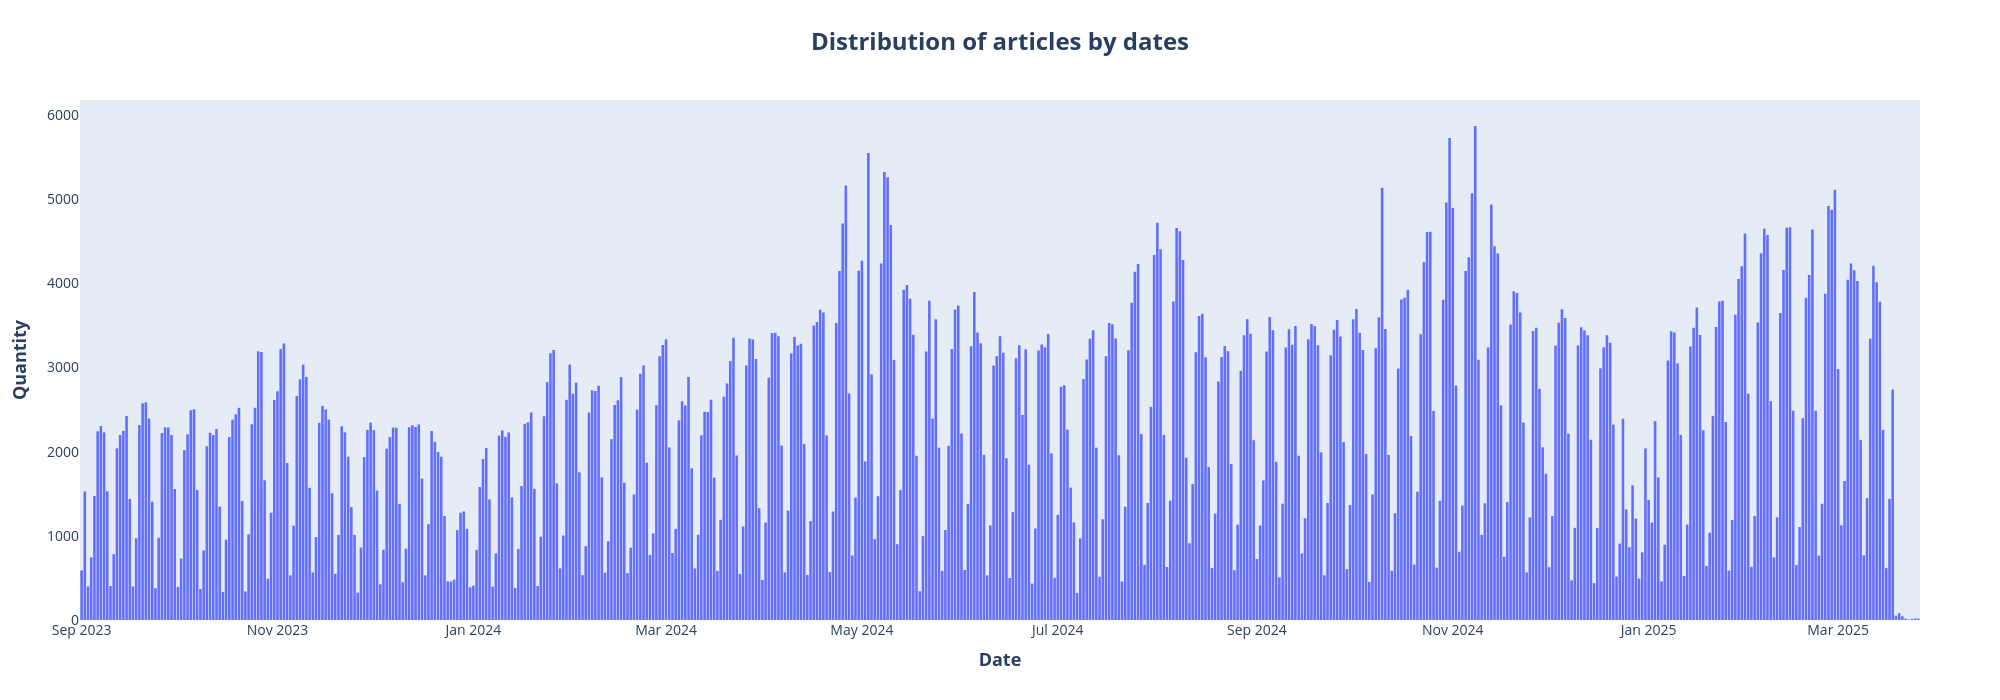
\includegraphics[width=1\linewidth]{img/articles_dist_by_dates.png}
    \caption{Distribution of publications by dates.}
    \label{fig:dist_by_dates}
\end{figure}

\textbf{Distribution of publications by dates.} Figure \ref{fig:dist_by_dates} shows that the number of publications
fluctuates daily with a certain periodicity. A detailed examination revealed that the minimums occur on Sundays and
public holidays, when fewer financial news items are published. This naturally reflects the market’s characteristics:
on weekends and holidays, business activity declines, leading to fewer publications.

\begin{figure}[H]
    \centering
    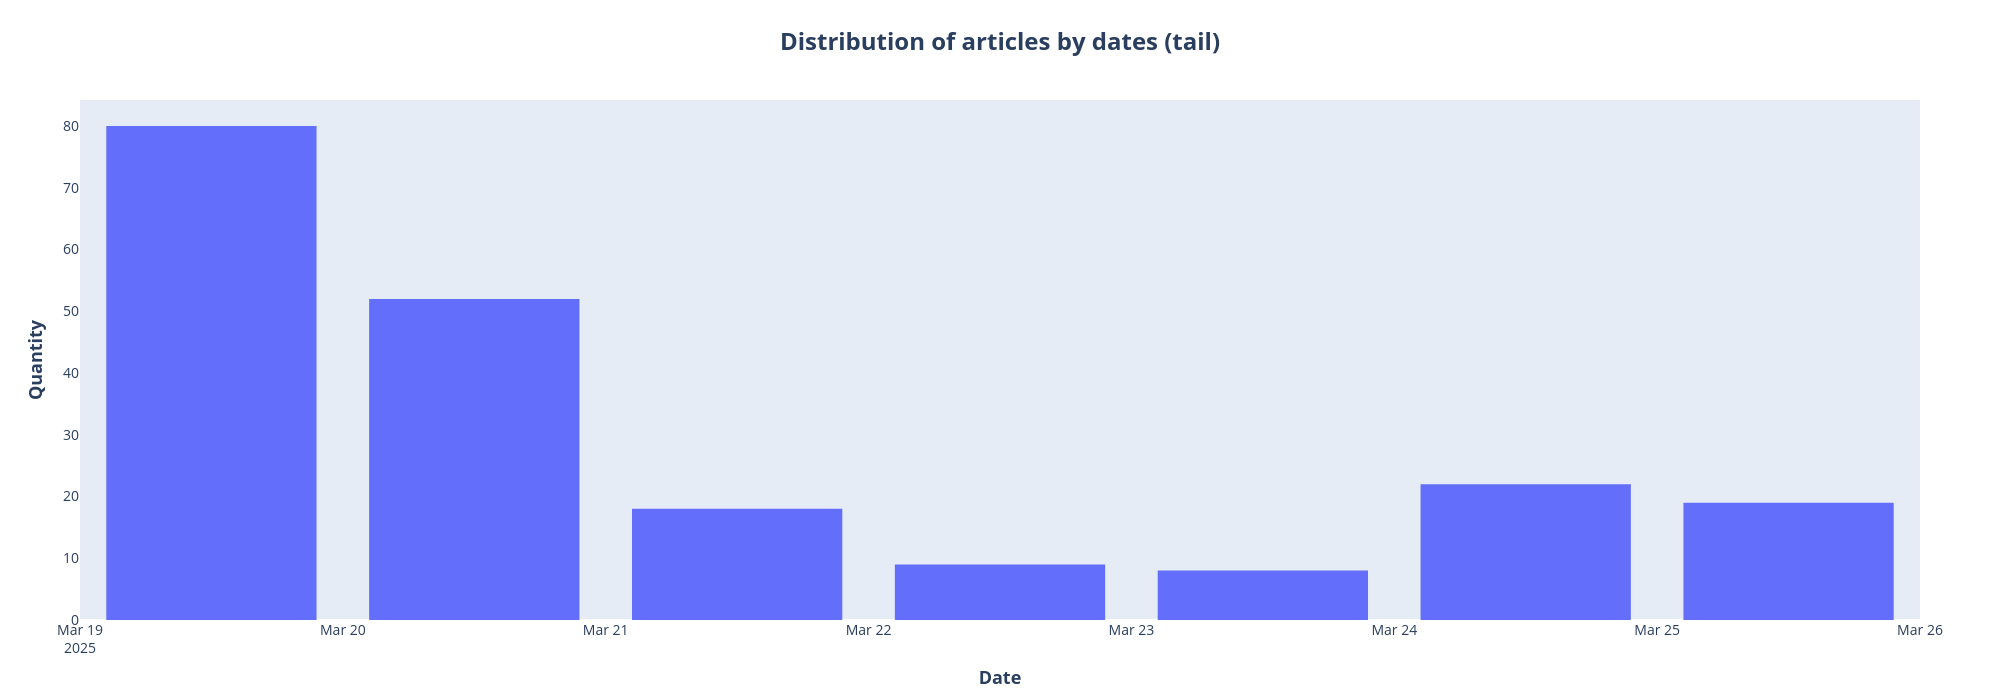
\includegraphics[width=1\linewidth]{img/articles_dist_by_dates_tail.png}
    \caption{\label{fig:dist_by_dates_tail}Distribution of publications by dates (tail).}
\end{figure}

At the same time, some articles, by formal characteristics, fall outside the collection period (September 17, 2023 - March 18, 2025).
Figure \ref{fig:dist_by_dates_tail} displays these "tail" publications, whose count slightly exceeds 200. A more detailed analysis
determined that these articles were indeed published within the specified interval, but their content was later edited or supplemented.
As a result, the publication date and time on the corresponding website were updated, and the old version (with the original date) was
lost. Had the links been parsed not after one week but several weeks later, more such cases would have been observed.

From the perspective of short-term market forecasting, this circumstance may lead to distorted timestamps, making some articles appear
to have been published later than they actually were. Therefore, the dataset might prove less effective for short-term studies compared
to medium- and long-term ones (where a shift of a couple of days is less critical). Nevertheless, for this work it does not play
a crucial role, as the model relies solely on the text of the article and does not take into account the precise publication timestamps.

\begin{figure}[H]
    \centering
    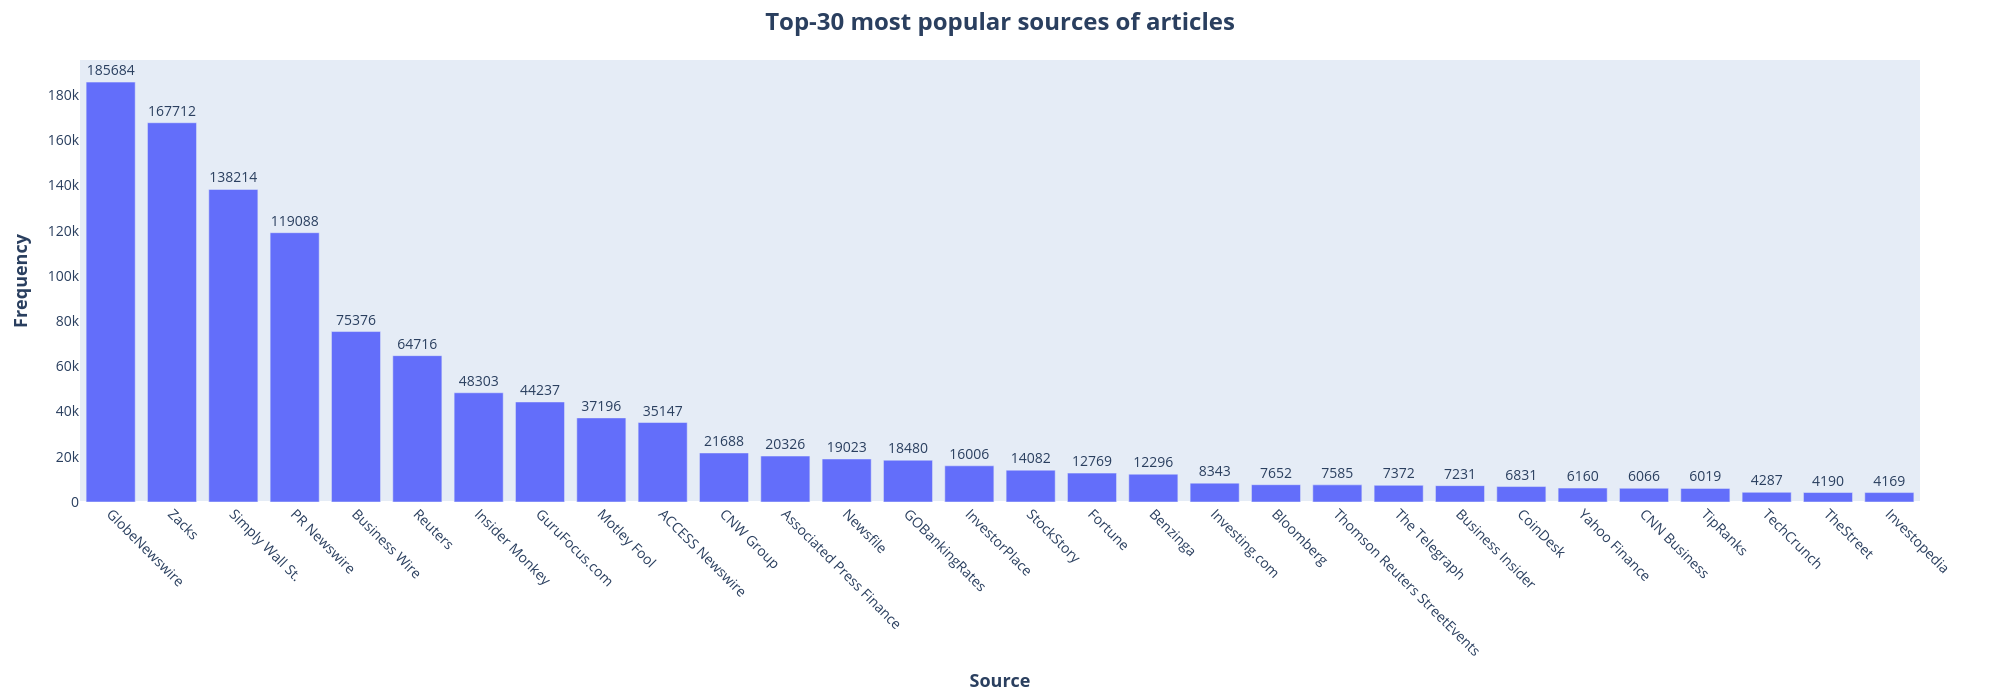
\includegraphics[width=1\linewidth]{img/top30_sources.png}
    \caption{\label{fig:dist_sources}Top-30 most popular sources of publications.}
\end{figure}

\textbf{News Sources.} Figure \ref{fig:dist_sources} illustrates the distribution of publications across the 30 most frequent sources.
The analysis showed that the predominant share of articles (potentially 69.2\%) was published by semi-automated aggregators:
GlobeNewswire, Zacks, Simply Wall St., PR Newswire, Business Wire, GuruFocus.com, Motley Fool, among others. These aggregators focus
on the automatic collection of key data from various resources (regulators, official company websites, etc.), publishing press releases,
brief report summaries, and invitations to corporate events.

Among the top 15 sources, only some can be conditionally considered as "traditional" news outlets, such as Reuters, Insider Monkey,
CNW Group, Associated Press Finance, and InvestorPlace. Meanwhile, outside the top 30, classic publications that primarily publish
original articles prevail. In reality, the blurred boundary between original and semi-automatically generated content complicates
efforts to clearly differentiate them.

According to approximate estimates, out of 1\,300\,000 articles, about 900\,000 (69.2\%) are semi-automated. This is an important factor
for training a language model because:

\begin{enumerate}
    \item The quality of such materials is often lower: texts contain artifacts, broken formatting, and incorrectly inserted characters.
    \item Their volume is large, which, on one hand, provides a substantial sampling capacity, but on the other, complicates cleaning and normalization without the loss of significant information.
\end{enumerate}

Nevertheless, even "imperfect" texts from aggregators convey useful information about the financial market and companies. However,
it is extremely important to develop appropriate cleaning and pre-processing rules (discussed in detail in \hyperref[sec:data_prep]{Section 2.2.4})
to preserve the semantic integrity of the texts.

Furthermore, and perhaps more importantly, these semi-automated texts contribute roughly the same total number of tokens
as the "original" articles (30.8\%), despite their numerical dominance. Consequently, with proper processing, this group of semi-automated
articles can make a significant contribution to training the language model without diminishing the value of the original texts.

\begin{figure}[H]
    \centering
    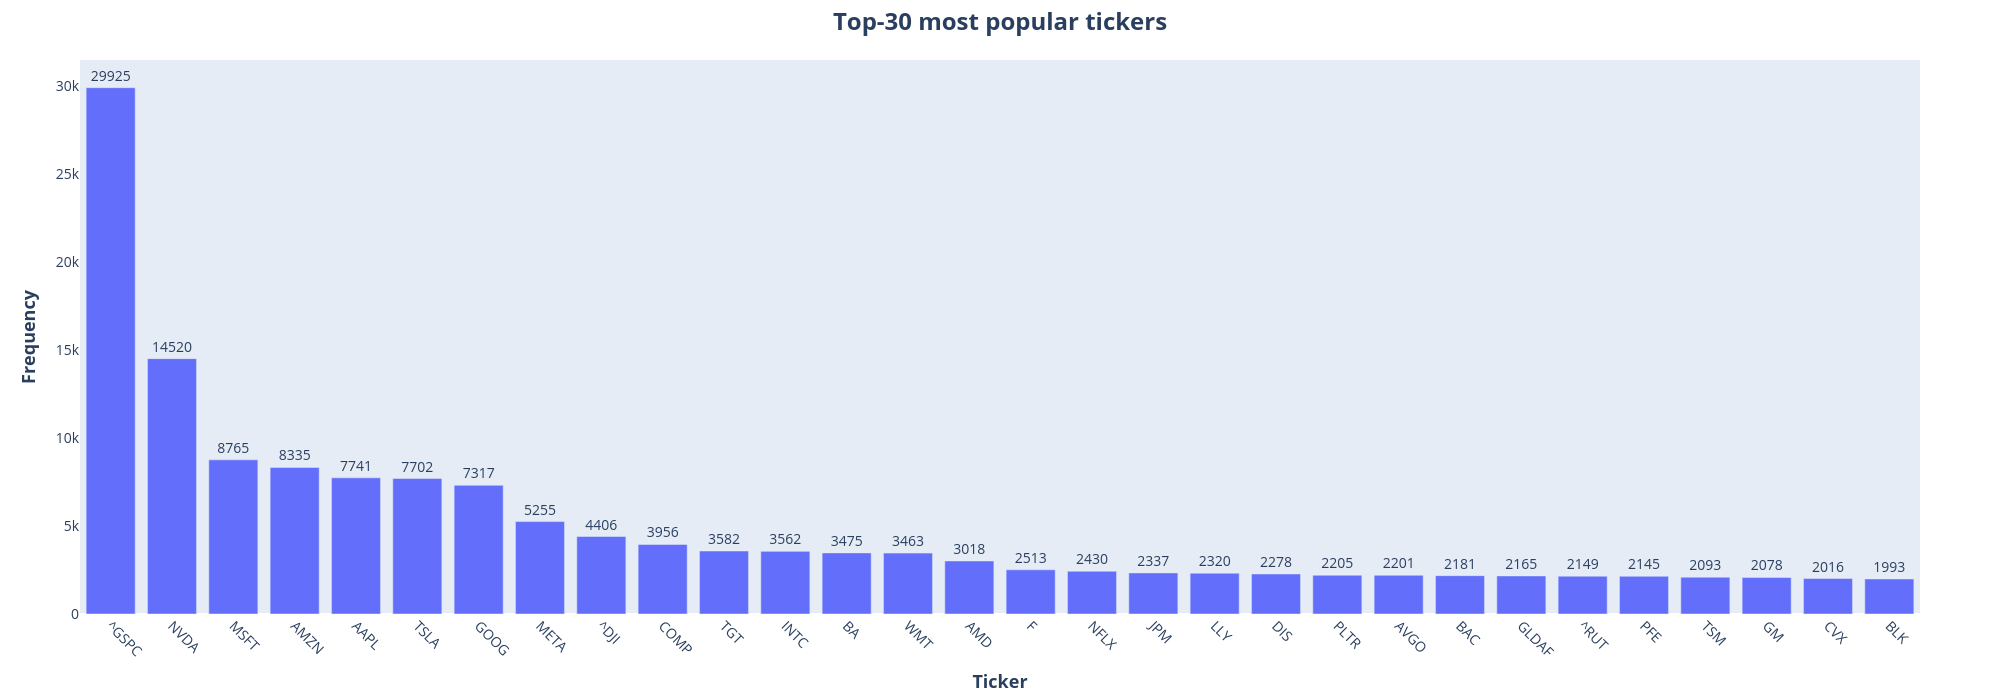
\includegraphics[width=1\linewidth]{img/top30_tickers.png}
    \caption{\label{fig:dist_tickers}Top-30 most popular tickers.}
\end{figure}

\textbf{Analysis of tickers.} Figure \ref{fig:dist_tickers} presents the distribution of publications by the 30 most frequently mentioned
tickers. The leader is the S\&P 500 index, although the sample also includes the Dow Jones and Russell 2000. Notably, the top 10 are predominantly
IT companies, with Nvidia leading by a significant margin.

At the same time, approximately 574\,000 (44.2\%) publications do not contain any tickers in the article header. Moreover, even when tickers
are present, they may not reflect all the companies or indices mentioned in the article. This indicates that although this dataset column
is fairly representative, it does not provide complete coverage of all potential tickers, and some news items are formally omitted
from consideration. Therefore, for tasks beyond the scope of this research, it would be advisable to create a dictionary of terms
and names associated with each specific ticker and then algorithmically augment the ticker column using the corresponding texts.

\begin{figure}[H]
    \centering
    
\includegraphics[width=1\linewidth]{img/wordcloud.png}
    \caption{\label{fig:wordcloud}Wordcloud of the whole collected corpus.}
\end{figure}

\textbf{Text Quality.} Figure \ref{fig:wordcloud} shows a word cloud generated from the entire corpus of collected texts.
From this visualization, the following key conclusions can be drawn:

\begin{enumerate}
    \item \textbf{Data Representativeness}. The word cloud demonstrates a wide range of financial terms, indicating that the dataset
    is sufficiently representative of financial topics. This suggests that the material covers various aspects of market activity
    and economic events.
    \item \textbf{Specificity of Financial Terminology}. The frequency distribution of financial terms significantly differs from that observed
    in popular corpora used for training language models (e.g., English Wikipedia or BookCorpus). This discrepancy necessitates the application
    of DAPT to effectively train the model on domain-specific financial data.
    \item \textbf{Level of Noise and Presence of Irrelevant Information}. The word cloud includes elements such as “Zacks”, “click”, “please”,
    “free”, and “source”. This indicates a significant presence of noisy, promotional, or automatically generated fragments, which calls
    for the development of specialized methods for data cleaning without compromising the semantic integrity of the texts.
\end{enumerate}

Additionally, it can be noted that the identified noise and dispersion of terms may negatively affect the quality of downstream tasks,
such as classification or embedding extraction, if the data is not properly processed during the pre-processing stage.

\textbf{Summary}. The collected news dataset is characterized by several notable features. Firstly, there is pronounced seasonality
in the publications—the minimums occur on weekends and public holidays, and so-called "tail" articles have also been recorded.
Secondly, the analysis of sources indicates that about 69\% of the texts originate from semi-automated aggregators, which can complicate
the data cleaning process, as such sources often yield texts with broken formatting, embedded artifacts, and irrelevant information.
Finally, it has been determined that the dataset exhibits a high variability of financial terminology while also containing a significant
level of noise, which altogether confirms the need for DAPT and the development of effective text cleaning
methods.

On one hand, the identified features (time shifts, noise, dominance of semi-automated sources) may reduce the suitability of the dataset
for short-term forecasting or tasks that require precise timestamping. On the other hand, for tasks oriented toward the semantic content
of the text, these issues do not have a critical impact. Proper pre-processing, including text cleaning and the removal of irrelevant
elements, will substantially improve the quality of the trained model and expand its ability to generalize across various types of publications.

\subsubsection{Data Preprocessing}
\label{sec:data_prep}
After local and global analyses of the text data, which revealed both noise patterns within individual documents and system anomalies
indicating the unrepresentativeness of some publications in the corpus as a whole, a multi-stage streaming on-the-fly preprocessing
pipeline was designed using chunks of 100,000 publications. A key limitation in the development of the solution was the limited
memory: with the original corpus size of about 15 GB, standard filtering and full text traversal operations required the allocation
of a significant constant memory buffer. This necessitated adapting the algorithm to stream processing in fixed-size chunks.

During the first stage, each chunk was downloaded from the repository and immediately subjected to initial filtering: documents
containing less than 100 characters were rejected as insufficiently informative. The empirically set threshold of 100 characters
turned out to be sufficient to eliminate “empty” artifacts arising due to markup instability on the source side. For example,
on popular sites like Yahoo! Finance, text is sometimes stitched inside atypical HTML tags — for example, in '<tbody>' instead
of the familiar '<p>' — resulting in almost entirely whitespace entries or marketing inserts at the end of the document.

The next step was to implement a headline filter: 66 rules were formalized based on it, covering both generic patterns ('Form 8',
'Net Asset Value', 'Holdings in company') and more targeted for noisy 12 sources (for example, GlobeNewswire removed headlines
containing 'Declaration' or starting with 'Key digital'). This selection ensured the removal of publications consisting
predominantly of tabular data or short fillers.

After normalizing all kinds of whitespace - merging consecutive spaces or line breaks into a single character, replacing unbroken
spaces '\\xa0' with a standard space, and unifying special characters in the text — 12 more rules were applied to reject
unrepresentative documents based on the content of the main body of the publication. In particular, anything starting with
the “(Repeat)” marker, as well as welcome templates of specific sources like “Dear madam, sir, please find hereunder the links”
for GlobeNewswire, were automatically excluded from further processing.

Next, the text was cleaned of contact information and typical footers: links, email addresses, and phrases that clearly indicate
the end of the document (“Forward-looking statements”, “Contact Details”) or the unrepresentativeness of a paragraph (“Source:”,
“See More:”, “Sponsored:”). In addition, standard introductory phrases such as “The recommendations of Wall Street analysts” and
“When deciding whether to buy, sell, or hold a stock, investors often rely on analyst recommendations” were removed from
the beginning of publications. A total of 92 cleaning rules were generated across the different groups.

This aggressive cleaning of texts is due to the fact that filtered patterns are so frequent that they have an extremely negative
impact on clustering, artificially inflating the clustering metric. After the aggressive cleaning of the corpus, the quality metric
did decrease, but the clusters became much more representative and based on the semantics of the news itself rather than its
sources, marketing and legal information in the texts.

\begin{figure}[H]
    \centering
    
\includegraphics[width=1\linewidth]{img/prep_wordcloud.png}
    \caption{\label{fig:prep_wordcloud} Wordcloud of the whole collected corpus after text and documents preprocessing.}
\end{figure}

As a validation of the quality of text cleaning, we can refer to the word cloud of the corpus after preprocessing
(Figure \ref{fig:prep_wordcloud}), which clearly shows the improvement: words such as 'forwardlooking', 'link', 'click', 'simply'
(source name Simply Wall St.) and others are missing.

Finally, before saving the chunks, sorting by publication date and deleting duplicates based on the full text of the document
took place. Taking into account the described operations, the size of the corpus was reduced from 15.4 GB in CSV format (8.6 GB
in Parquet) to 5.9 GB (2.0 GB in Parquet): out of 1,304,717 original records, 1,267,416 remained, i.e., only 2.8\%
of the documents were deleted. This result indicates a high proportion of text noise in the collected dataset and emphasizes
the effectiveness of the multi-stage stream-based preprocessing approach, which saves RAM and provides high-quality cleaning
of text data before subsequent stages of thematic modeling and analysis.


\subsection{Model Development}
\subsubsection{Feature Extraction}
After preprocessing the text corpus and removing background noise, embeddings were extracted
to accelerate subsequent stages of topic modeling, including dimensionality reduction and clustering.

The base ModernBERT model is not optimal for this task, since its vector representations are excessively
sparse. High sparsity of embeddings degrades clustering quality, particularly for density-based methods
(e.g., DBSCAN). Although HDBSCAN is more robust to density variations, sparsity still adversely affects
clustering outcomes.

To address this issue, it is common to fine-tune the model on a semantic textual similarity (STS) task.
In this setting, the model receives a pair of texts and returns a similarity score \parencite{MTEB2023},
typically computed via cosine distance (Formulation \ref{eq:cos_dist}).

\begin{equation}\label{eq:cos_dist}
    D_{\cos}(\mathbf{u}, \mathbf{v})
    = 1 - \frac{\mathbf{u} \cdot \mathbf{v}}
                 {\|\mathbf{u}\|_2 \,\|\mathbf{v}\|_2}.
\end{equation}

STS models consistently produce denser and more informative embeddings.

Accordingly, for the base ModernBERT we evaluated two fine-tuned variants: modernbert-embed from Nomic AI
\parencite{nomic2024} and gte-modernbert-base from Alibaba \parencite{MGTE2023,MGTE2024}. Evaluation
employed the Massive Text Embedding Benchmark (MTEB), which spans eight task categories and 58 datasets
\parencite{MTEB2023}. Results were as follows:

\begin{itemize}
    \item Clustering (12 datasets): gte-modernbert-base outperformed modernbert-embed by 1.5 percentage
    points (44.98\% vs. 44.47\%).
    \item STS (10 datasets): Their performances were comparable (81.78\% vs. 81.57\%).
    \item Overall (eight tasks, 56 datasets): gte-modernbert-base led by 1.76 percentage points on average
    (64.38\% vs. 62.62\%).
\end{itemize}

Consequently, gte-modernbert-base from the sentence\_transformers library was chosen for embedding extraction
\parencite{SBERT2019}. Instead of using the [CLS] token, a more advanced Mean Pooling technique was applied,
averaging token embeddings across the sequence (Formulation \ref{eq:mean_pooling}).

\begin{equation}\label{eq:mean_pooling}
    \mathbf{h_{mean}}=\frac{1}{T}\sum^T_{t=1}\mathbf{h}_{t}.
\end{equation}

where $T$ is the tokenized sequence length and $\mathbf{h}_t$ denotes the embedding of the $t$-th token.

To accelerate the training of dimensionality reduction and clustering models, the embeddings were
first reduced to the unit $L_2$-norm (Formulation \ref{eq:l2_norm}):

\begin{equation}\label{eq:l2_norm}
    \widehat{\mathbf{u}}
    = \frac{\mathbf{u}}{\|\mathbf{u}\|_2},
    \qquad
    \|\mathbf{u}\|_2 = \sqrt{\sum_{i=1}^{n} u_i^2}.
\end{equation}

Such preprocessing allows us to use the GPU-optimized Euclidean distance metric (Equation \ref{eq:euclidean})
when training the dimensionality reduction model, without having to repeat the $L_2$-norm computation that
occurs when computing the cosine distance metric at each iteration of the hyperparameter optimization.
so that Euclidean distance could be used for both dimensionality reduction and clustering.

\begin{equation}\label{eq:euclidean}
    D_{2}(\mathbf{u}, \mathbf{v})
    = \|\mathbf{u} - \mathbf{v}\|_2
    = \sqrt{\sum_{i=1}^{n} \bigl(u_i - v_i\bigr)^2}.
\end{equation}

Thus, after computing the $L_2$-norm and the Euclidean distance, we can actually, in a sense, be considered
to be working with the cosine distance, since the reduced measure becomes monotonically related to the cosine
and reflects the same order of proximity of the points (Equation \ref{eq:euclidean_after_l2_norm}), but all
computations are accelerated by GPU optimization.

\begin{equation}\label{eq:euclidean_after_l2_norm}
    D_{2}\bigl(\widehat{\mathbf{u}}, \widehat{\mathbf{v}}\bigr)
    = \bigl\|\widehat{\mathbf{u}} - \widehat{\mathbf{v}}\bigr\|_2
    = \sqrt{2\,\bigl(1 - \widehat{\mathbf{u}}\!\cdot\!\widehat{\mathbf{v}}\bigr)}.
\end{equation}

To build and train the dimensionality reduction and clustering algorithms, a training subsample of 200,000 embeddings
and associated metadata was generated, which is approximately 16\% of the entire corpus. This size of the training
subsample was chosen based on the available computational resources. Thus, 200,000 embeddings were used to select
the optimal hyperparameters, while the remaining 1,050,000 embeddings were reserved for the validation and inference
phases. At the same time, before inference, the pipeline of dimensionality reduction and clustering models were trained
on the entire corpus with a linear increase in hyperparameter values for the HDBSCAN algorithm, the choice of which
is conditioned in \hyperref[sec:drc]{Section 2.3.2}.

Moreover, mixed precision (float16) and the FlashAttention mechanism \parencite{flash2022attention} were
employed during embedding extraction, substantially reducing computational resource requirements and runtime.

\subsubsection{Dimensionality Reduction and Clustering}
\label{sec:drc}
Thus, after assembling the embedding sample, we proceeded to experiments with dimensionality reduction and clustering
models, performing their joint optimization. This approach reflects the multi-criteria nature of the task: it is necessary
not only to preserve the structural (global) and local relationships from the original 768-dimensional space, but also
to ensure that embeddings remain separable (“clusterable”) in a low-dimensional projection suitable for two-dimensional
visualization.

As key requirements we identified:

\begin{enumerate}
    \item Preservation of cluster structure. Embeddings after dimensionality reduction must remain separable,
    preserving groupings by semantic and topical similarity.
    \item Suitability for two-dimensional visualization. The resulting space must support clear and interpretable
    planar display.
\end{enumerate}

To search simultaneously for optimal hyperparameters of both dimensionality reduction algorithms and clustering methods,
we employed a unified meta-optimization process.

We used the DBCV index as our optimization metric, since it does not assume any predefined cluster shape (unlike as example
silhouette coefficient favoring spherical or ellipsoidal structures) and effectively evaluates density-based clustering
methods.

As our base clustering algorithm we selected HDBSCAN \parencite{HDBSCAN2013}, which meets two crucial requirements:

\begin{itemize}
    \item No shape assumptions. Unlike K-Means, HDBSCAN does not assume clusters are Gaussian spheres, which is critical
    for representing topics.
    \item Hierarchical, density-based nature. It can identify both large thematic groups and small, highly concentrated niches.
\end{itemize}

Moreover, GPU acceleration of HDBSCAN yielded high processing speed on both large samples and high-dimensional data.

Within the HDBSCAN framework, we tuned two key hyperparameters: the minimum number of neighbors --- the count of points
in a neighborhood required to consider a point a cluster “core” --- and the minimum cluster size --- the threshold number
of observations for forming a cluster, which allows capturing rare, narrowly topical groups.

Pilot experiments revealed the coexistence of very dense regions (“hot topics”) and rare but semantically significant
clusters. A small minimum cluster size captures these rare topics but also increases the number of micro-clusters,
some of which lack clear semantic distinction.

To mitigate this, we considered an $\epsilon$-based cluster-merging technique \parencite{HDBSCAN2020cluster_selection_epsilon},
consolidating adjacent micro-clusters in high-density regions. However, this approach complicates inference: when new
observations arrive, $\epsilon$-merging cannot be incrementally updated, necessitating full retraining.

Prioritizing practicality, we therefore abandoned $\epsilon$-merging in favor of smaller minimum cluster sizes, accepting
some fragmentation while preserving the ability to interpret and agglomerate clusters at higher hierarchical levels.

Another hyperparameter --- the cluster selection method --- determines whether clusters form based on excess of mass
or tree leaves. We found that the latter yields finer-grained, more homogeneous groups, and used it for our final
configuration.

Thus, in the final optimization stage, only two HDBSCAN parameters remained tunable: minimum neighbors and minimum cluster
size.

It is noteworthy that, as will be described in \hyperref[sec:architecture]{Section 3.3}, the future architecture assumes
a fixed number of clusters corresponding to a static number of experts; hence, we employ the cuML implementation of HDBSCAN
rather than its adaptive variant \parencite{HDBSCAN2022adaptive}.

Turning to dimensionality reduction algorithms, our preliminary selection included t-SNE, PCA, UMAP, TriMap, and PaCMAP,
with key evaluation criteria of fidelity, the ability to balance local and global relationships, and training time complexity.
Based on other researchers' experience, UMAP was chosen as the baseline algorithm \parencite{BERTopic2022}.

t-SNE was excluded due to its insufficient scalability on large datasets. PCA, although fast as a global approximation,
did not preserve local structure in the final low-dimensional embedding, and an experiment combining PCA with UMAP fell
short of standalone UMAP by approximately 37\% in DBCV score. While TriMap and PaCMAP achieved similar performance
in intermediate dimensions --- and PaCMAP produced a more uniform distribution for two-dimensional visualization ---
the GPU-accelerated implementation and demonstrated robustness of UMAP in cuML led us to select it as the definitive method
for both intermediate dimensionality reduction and final 2D projection.

\subsubsection{Hyperparameters Optimization}
<<To be done later>>

\subsection{System Development}
<<To be done later>>

    % Третья результирующая глава
    \newpage
    \section{РАЗУЛЬТАТЫ}
    \label{sec:results}
    \subsection{Invented Architecture}
\label{sec:architecture}
\subsubsection{Overview}
<<To be done later>>

\subsubsection{Embedding System}
<<To be done later>>

\subsubsection{Aspect-Based Sentimental Block}
<<To be done later>>

\subsubsection{Feature Caching Machine (FCM)}
<<To be done later>>

\subsection{Finished System Components}
\subsubsection{Эмбеддинговая система и роутер}
\label{sec:emb_sys_and_router}

Основным итогом настоящего исследования стало создание двух ключевых компонентов: гибкой эмбеддинговой подсистемы
и обучаемого роутера для блока MoTE. Эти наработки не только обеспечивают надёжный фундамент для дальнейшего
развития FinABYSS, но и открывают широкий простор для применения в смежных прикладных проектах.

В рамках исследования мы провели серию экспериментов по отбору оптимальных комбинаций эмбеддинговых моделей,
методов понижения размерности и алгоритмов кластеризации, используя разные метрики для настройки гиперпараметров.
На первом этапе базовая цепочка состояла из ModernBERT, UMAP (косинусная метрика), HDBSCAN (эвклидова метрика)
оптимизировалась по коэффициенту силуэта. Несмотря на удовлетворительные результаты, мы отметили сильную
зависимость от структуры кластеров и чувствительность силуэта к форме кластеров.

Второй этап повторил ту же связку, но в качестве целевой метрики был выбран DBCV-индекс. Благодаря свойству
DBCV учитывать плотностные особенности и неоднородность распределения точек, гиперпараметры, подобранные
под DBCV, обеспечили более семантически согласованные и плотные кластеры.

Наконец, мы протестировали тонко настроенную на задачу STS версию ModernBERT ('gte-modernbert-base') \parencite{Warner2024ModernBERT, MGTE2024} в сочетании с UMAP,
но уже с $L_2$–эвклидовой метрикой, и тем же HDBSCAN, также настроенным под $L_2$–евклидову дистанцию (Таблица \ref{tab:experiment_configs}).
днако это сочетание уступило предыдущему: полученный DBCV-индекс составил лишь 0.405 против 0.476 у пары "cosine + euclidean" (Таблица \ref{tab:experiment_results}).

\begin{longtable}[c]{|l|ll|}
    \caption{Description of the final configurations of experiments conducted on a subsample of 10,000 embeddings.}
    \label{tab:experiment_configs}\\
    \hline
    \multicolumn{1}{|c|}{\multirow{2}{*}{\textbf{Model}}} & \multicolumn{2}{c|}{\textbf{Configuration}}                         \\ \cline{2-3}
    \multicolumn{1}{|c|}{}                                 & \multicolumn{1}{c|}{(I)}               & \multicolumn{1}{c|}{(II)}  \\ \hline
    \endfirsthead

    \endhead

    UMAP    & \multicolumn{1}{l|}{$L_2$-Euclidean} & \multicolumn{1}{l|}{Cosine}    \\
    HDBSCAN & \multicolumn{1}{l|}{$L_2$-Euclidean} & \multicolumn{1}{l|}{Euclidean} \\ \hline
\end{longtable}

Дополнительный анализ шумовых точек и структуры кластеров не подтвердил это преимущество (Таблица \ref{tab:experiment_results}),
однако в ходе анализа выяснилось, что подобная ситуация просиъодит по причине внутренней нестрабильности GPU реализации \parencite{cuml2020machine}. На метрике же,
данный факт не сказался существенно негативным образом. При использовании $L_2$–метрики
доля шумовых точек достигала 39.54\%, число кластеров --- 73 (при максимальном размере 3 824 точек и минимальном --- 365).
Для пары "cosine + euclidean" больше точек было отмечено как шум 43.38\%, а число кластеров увеличилось до 141; при этом максимальный
кластер вырос до 2 558 точек, а минимальный сократился до 147. Так как целевая метрика именно DBCV, можно сделать вывод, что
подход "cosine + euclidean" продемонстрировал лучшую устойчивость кластеров.

% Please add the following required packages to your document preamble:
% \usepackage{multirow}
% \usepackage{longtable}
\begin{table}[!htbp]
\begin{longtable}[c]{|cl|cc|}
    \caption{Summary table of the results of hyperparameter optimization performed for three specified configurations on a subsample of 10,000 embeddings.}
    \label{tab:experiment_results}\\
    \hline
    \multicolumn{2}{|c|}{\multirow{2}{*}{\textbf{Best trial}}} & \multicolumn{2}{c|}{\textbf{Configuration}}                                                \\ \cline{3-4}
    \multicolumn{2}{|c|}{}                                     & \multicolumn{1}{c|}{(I)} & \multicolumn{1}{c|}{(II)} \\ \hline
    \endfirsthead

    \endhead

    \hline
    \endfoot

    \endlastfoot

    \multicolumn{1}{|c|}{\multirow{7}{*}{\textbf{Hyperparameters}}} & n\_components            & \multicolumn{1}{c|}{47}                & \multicolumn{1}{c|}{41}             \\
    \multicolumn{1}{|c|}{}                                          & n\_neighbors             & \multicolumn{1}{c|}{70}                & \multicolumn{1}{c|}{75}             \\
    \multicolumn{1}{|c|}{}                                          & min\_dist                & \multicolumn{1}{c|}{0,0}               & \multicolumn{1}{c|}{0,065}          \\
    \multicolumn{1}{|c|}{}                                          & spread                   & \multicolumn{1}{c|}{6,5}               & \multicolumn{1}{c|}{6,4}            \\
    \multicolumn{1}{|c|}{}                                          & negative\_sample\_rate   & \multicolumn{1}{c|}{10}                & \multicolumn{1}{c|}{11}             \\
    \multicolumn{1}{|c|}{}                                          & min\_cluster\_size       & \multicolumn{1}{c|}{360}               & \multicolumn{1}{c|}{145}            \\
    \multicolumn{1}{|c|}{}                                          & min\_samples             & \multicolumn{1}{c|}{180}               & \multicolumn{1}{c|}{170}            \\ \hline
    \multicolumn{1}{|c|}{\multirow{5}{*}{\textbf{Statistics}}}      & Max cluster size         & \multicolumn{1}{c|}{3824}              & \multicolumn{1}{c|}{2558}           \\
    \multicolumn{1}{|c|}{}                                          & Min cluster size         & \multicolumn{1}{c|}{365}               & \multicolumn{1}{c|}{147}            \\
    \multicolumn{1}{|c|}{}                                          & Total clusters           & \multicolumn{1}{c|}{73}                & \multicolumn{1}{c|}{141}            \\
    \multicolumn{1}{|c|}{}                                          & Noise \%                 & \multicolumn{1}{c|}{\textbf{39,54\%}}  & \multicolumn{1}{c|}{43,38\%}        \\
    \multicolumn{1}{|c|}{}                                          & DBCV Index               & \multicolumn{1}{c|}{0,397}             & \multicolumn{1}{c|}{\textbf{0,407}} \\ \hline
\end{longtable}
\end{table}

Экспериментальные результаты однозначно свидетельствуют о превосходстве схемы ModernBERT + UMAP
с косинусной метрикой и HDBSCAN с эвклидовой дистанцией в задачах тематической кластеризации
финансовых текстов. В сочетании с оптимизацией по DBCV-индексу данный подход формирует наиболее
семантически связные группы, минимизирует долю шумовых экземпляров и предоставляет более стабильную
основу для последующего обучения роутера MoTE.

Тем не менее, к сожалению, были выявлены и явные проблемные места текущей реализации.
Полученные кластеры и их структура не могут инкрементально обновляться при потоковых
поступлениях новых публикаций, что происходит по нескольким причинам. Во-первых, обученная
модель является GPU-реализацией из библиотеке 'cuML', в которой лишь после проведения исследования
были обнаружены критические ошибки в коде версии 25.02 \parencite{cuml2020machine}. Во-вторых, выбранный
алгоритм UMAP достаточно плохо работает в инкрементальном режиме по своей природе, именно
поэтому существуют другие реализации, как например AlignedUMAP \parencite{mcinnes2018umap-software}
или ParametricUMAP, основанный на нейронной сети в качестве базовой модели \parencite{ParametricUMAP2020}.
К сожалению, обе данные реализации доступны исключительно для обучения на центральном, а не графическом процессоре.
А для обучения на центральном процессоре в контексте текущего исследования недостаточно вычислительных ресурсов.

Таким образом, узким местом данного исследования и предложенного решения является недостаток вычислительных
мощностей для обучения моделей, что будет доработано в дальнейших исследованиях.

\subsubsection{Семантическая карта}

Наконец, на базе разработанной эмбеддинговой подсистемы и роутера MoTE была обучена отдельная модель UMAP,
призванная переводить векторы из промежуточного латентного пространства кластеризации в двумерное представление,
удобное для визуального анализа. Именно эта проекция лежит в основе Семантической карты финансовых публикаций ---
одного из ключевых компонентов интерфейса FinABYSS, обеспечивающего глубокое и интуитивно понятное исследование
тематической структуры новостных потоков.

\begin{figure}[H]
    \centering
    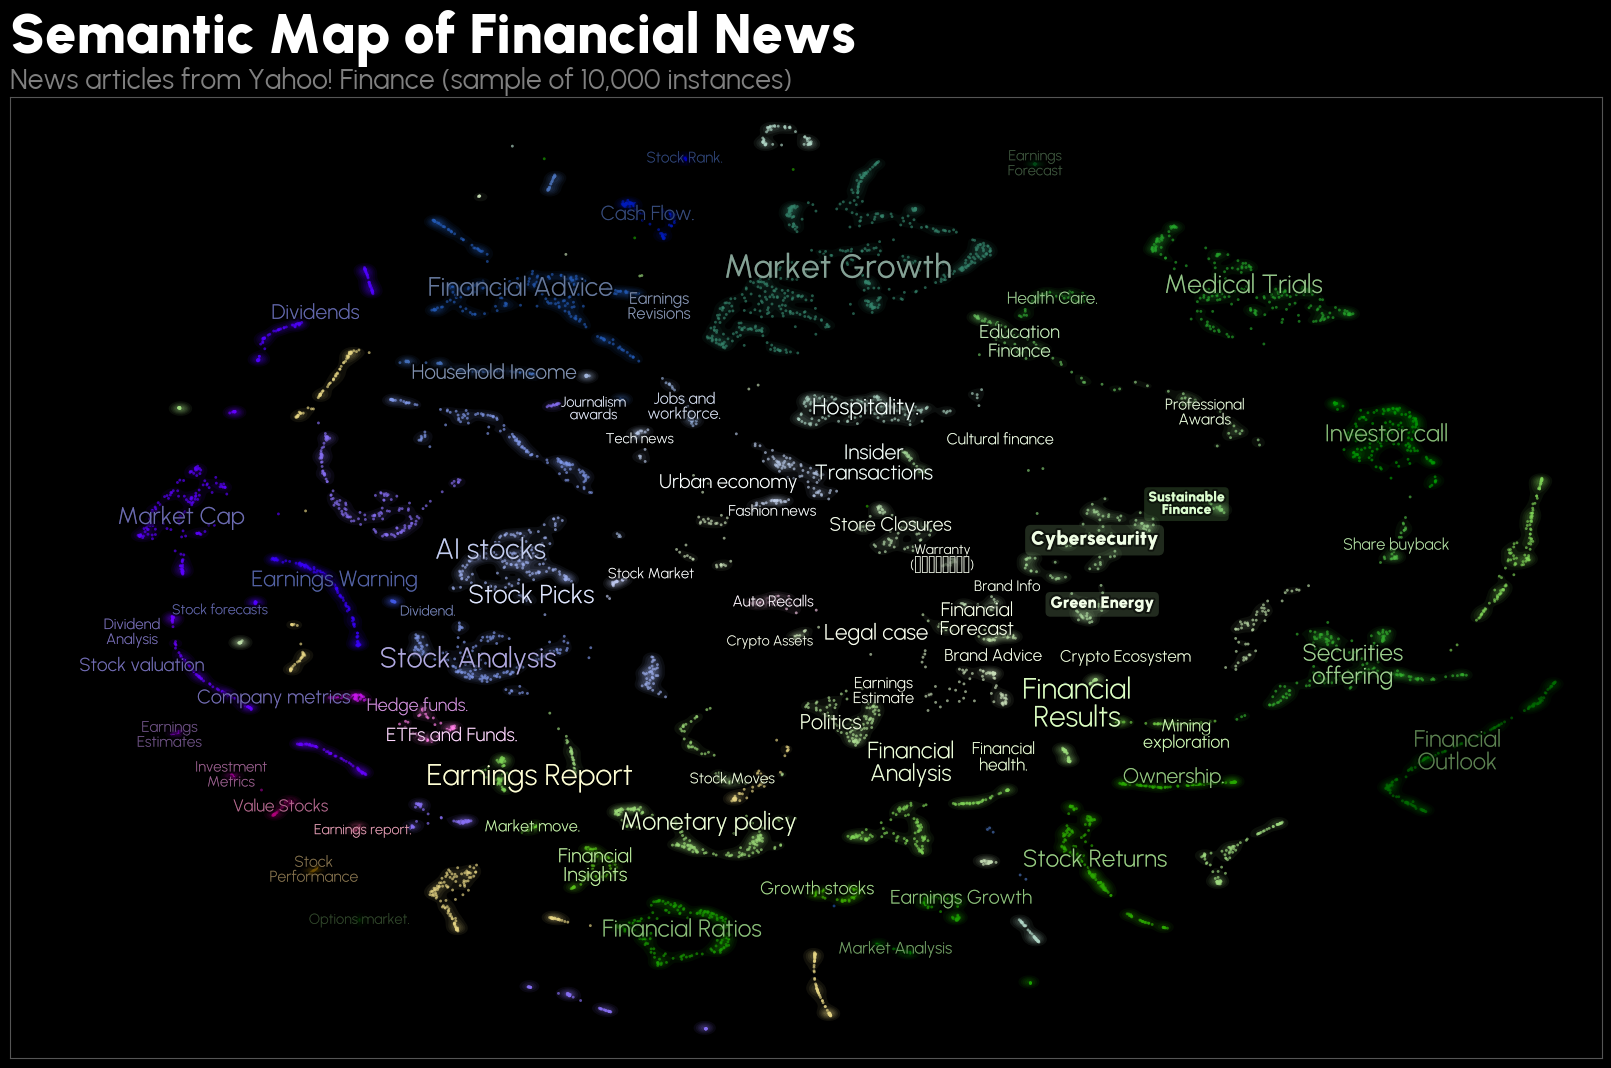
\includegraphics[width=1\linewidth]{img/semantic_map.png}
    \caption{Статичная семантическая карта, разработанная на основе подвыборки из 10 000 финансовых публикаций,
    опубликованных в период с 17.09.2023 по 18.04.2025, и кластеризованных по темам.}
    \label{fig:semantic_map}
\end{figure}

Для начала была реализована статическая версия карты, на которой отображены 100 000 финансовых статей за период
с сентября 2023 по март 2025 года, разбитые на кластеры по тематике (Изображение \ref{fig:semantic_map}).
Каждый кластер промаркирован автоматически сгенерированным словом-меткой без какой-либо ручной аннотации.
Несмотря на автоматический характер присвоения, метки получились репрезентативными: плотные группы статей,
посвящённые здравоохранению, «Устойчивым финансам», «Кибербезопасности» и «Зелёной энергетике», расположены
рядом, что отражает их семантическую близость; аналогично происходит с кластерами «Политика» и «Монетарная политика».

Однако статическая карта демонстрирует потенциал лишь UMAP-проекции. Интерактивная Семантическая
карта FinABYSS выходит далеко за рамки простой визуализации точек:

\begin{itemize}
    \item Наведение курсора на любую точку раскрывает метаданные статьи: заголовок, дата и время публикации,
    иерархическую тему (макро–/мезо–/микротема), автора и источник. При этом доступен предпросмотр полного
    текста и прямая ссылка на оригинал публикации.
    \item Механизм поиска по ключевым словам позволяет быстро отфильтровать статьи, содержащие специальные термины.
    Поиск можно комбинировать с фильтрами по диапазону дат, объёму публикаций и другим числовым признакам (например,
    объёму текста или количеству просмотров), что облегчает точечное обнаружение исторических событий и триггеров
    на графике.
    \item Раздел источники и темы даёт возможность включать и исключать источники новостей или целевые кластеры,
    помогая сфокусироваться на релевантных публикациях в сложных аналитических сценариях.
    \item Также для статей доступна функция облака слов, формируемого на основе наиболее частых слов, встречающихся
    в выделанной группе текстов. Облако слов мгновенно отображает доминирующие термины и паттерны обсуждения,
    что дополняет количественную канву графика качественными характеристиками.
\end{itemize}

Таким образом, Семантическая карта FinABYSS представляет собой полноценную аналитическую систему,
объединяющую мощь выбранных моделей UMAP и HDBSCAN, а при дальнейшем развитии и гибридной CNN-LSTM-архитектуры
и MoE-подхода к оценке тональностей. Она обеспечивает исследователю возможность не только визуально различать
именованные кластеры и их взаимное расположение, но и глубоко погружаться в содержание каждой публикации,
комбинируя автоматические и ручные методы анализа.

Разработанная интерактивная Семантическая карта выступает естественным продолжением предыдущих модулей FinABYSS.
Все звенья конвейера связаны в единую цепь. Инструмент предлагает пользователю прозрачный, масштабируемый
и гибко настраиваемый интерфейс для семантического исследования финансовых новостей, где каждый элемент ---
от кластерных меток до облака слов — отражает результаты вычислительной логики системы и поддерживает экспертные
решения при анализе рыночных процессов.

\subsubsection{Динамическое тематическое моделирование}

Помимо семантической карты, FinABYSS предоставляет мощный инструментарий для анализа лингвистических
особенностей сформированных тематических групп и динамического темпорального моделирования тем.
Все входящие тексты проходят описанный в \hyperref[sec:sys_dev]{Разделе 2.4} пайплайн постобработки в контексте Аналитического
GUI (см. \hyperref[sec:sys_dev]{Раздел 3.1.6}), где каждому документу присваивается превалирующая тема,
а затем извлекаются и агрегируются соответствующие лексические признаки.

Так, система визуализирует частотное распределение самых релевантных слов в рамках выбранной темы
(Изображение \ref{fig:topics_words_freqs}). Такая лингвистическая панель служит двум целям:

\begin{itemize}
    \item Во-первых, это позволяет после разработки системы в ручном режиме провалидировать качество сформированных
    тем и оценить насколько они уникальны и семантически однородны.
    \item Во-вторых, эта функциональность может быть весьма полезна при первичном знакомстве финансового аналитика
    с системой. Финансовый аналитик, впервые работающий с FinABYSS, мгновенно получает представление о содержании каждой темы без глубокого ознакомления с самими текстами.
\end{itemize}

Именно последний факт послужил причиной включения данной функциональности в набор основных инструменты GUI.

\begin{figure}[H]
    \centering
    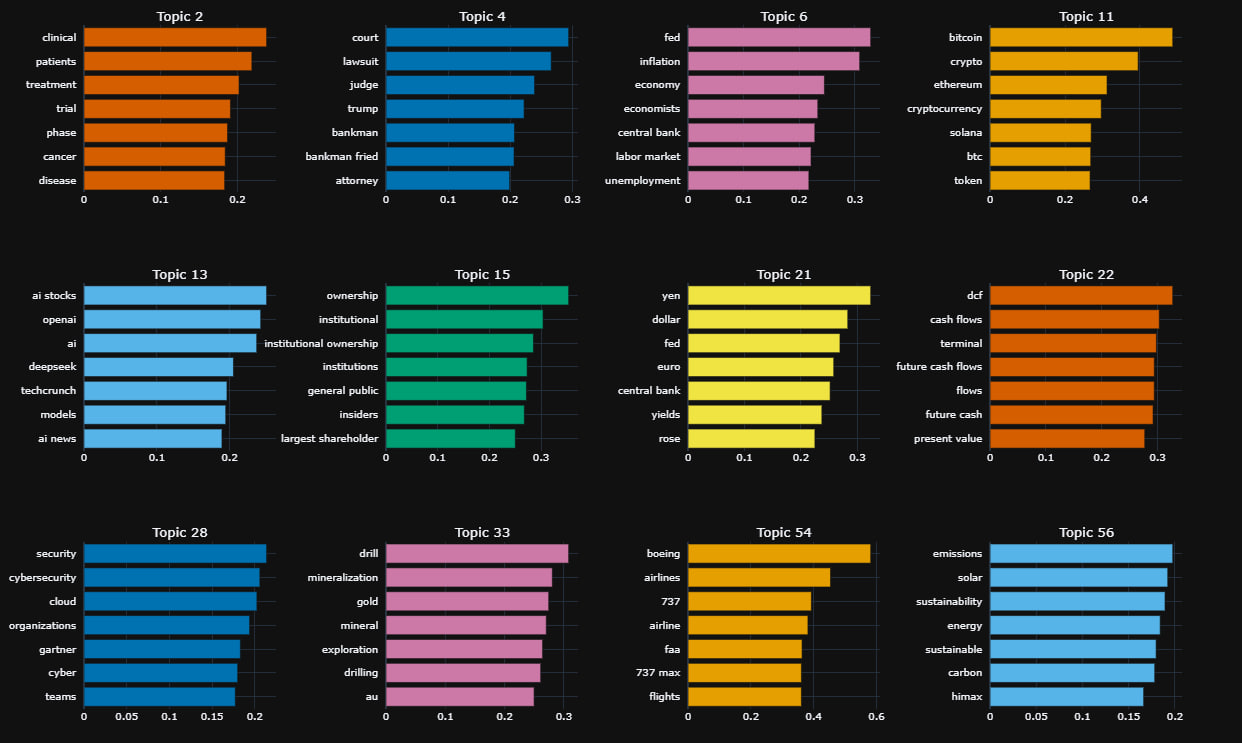
\includegraphics[width=1\linewidth]{img/topics_words_freqs.png}
    \caption{Ранжированные по релевантности термины выборки из 12 тем.}
    \label{fig:topics_words_freqs}
\end{figure}

Для иллюстрации данного функционала случайным образом была сформирована выборка из
125 000 публикаций, внутри которых было выбрано 12 тем для отображения. Среди выборки
все темы несомненно несут прикладное значение для финансовых рынков. Причем есть
более общие отраслевые темы, такие как:

\begin{itemize}
    \item Тема №2, связанная с фармацевтической отраслью;
    \item Тема №13, связанная с сектором искуственного интеллекта;
    \item Тема №28, связанная с кибербезопасностью;
    \item Тема №33, связанная с горнодобывающей отраслью;
    \item Тема №54, связанная с авиационной промышленностью.
\end{itemize}

С другой стороны в выборку попала и достаточно общая тема, которая стоит на повестке дня в том числе и в финансах ---
Тема №56, которая явно относится к ESG. Наконец, есть и узкоспециализированные финансовые темы,
которые также были выявлены автоматически:

\begin{itemize}
    \item Тема №4, связанная с судебными процессами и разбирательствами, потенциально она
    является крайне влиятельной в контексте ценообразования стоимости актива;
    \item Тема №6, связанная с внешнеэкономическими факторами и экономикой, в целом;
    \item Тема №11, напрямую связанная с рынком активов, а именно криптовалют;
    \item Тема №15, связанная с правами собственности, то есть держателями аккий компаний;
    \item Тема №21, связанная с валютным рынком;
    \item Тема №22, связанная с денежными потоками, включая будущие, настоящие и дисконтированные.
\end{itemize}

Так, мы можем наблюдать за лингвистическими особенностями тематических групп,
а также крайне быстро и эффективно изучать как различия между ними, так и конкретные темы вглубь.

С другой стороны, было бы крайне полезно понимать как темы меняются сквозь время, ведь информационное медиапространство
крайне нестабильно, а повестка дня в современном обществе меняется мгновенно. Так, FinABYSS реализует
динамическое тематическое моделирование через интерактивный график тематических временных рядов.

\begin{figure}[H]
    \centering
    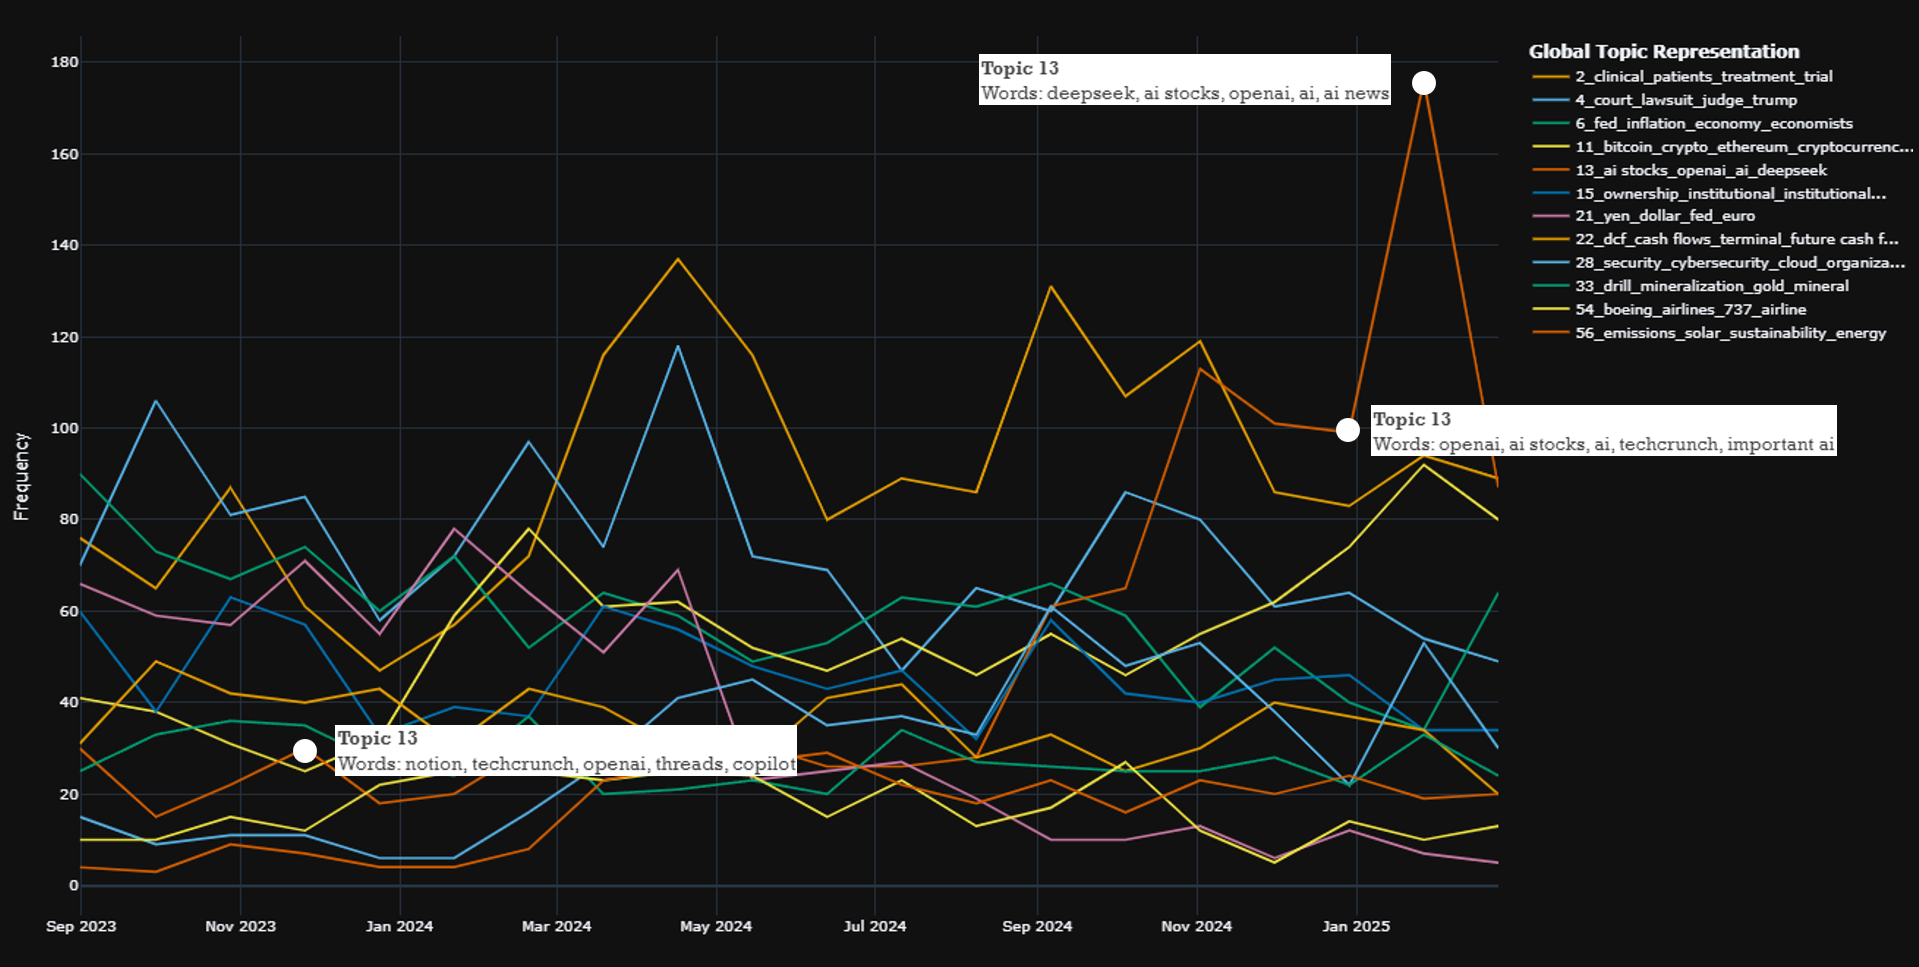
\includegraphics[width=1\linewidth]{img/dynamic_topic_modeling.png}
    \caption{Эволюционное тематическое моделирование и наиболее релевантные термины выборки из 12 тем за период с 17.09.2023 по 18.04.2025.}
    \label{fig:dtm}
\end{figure}

На Изображении \ref{fig:dtm} представлена та же выборка из 12 тем. Ось абсцисс отражает интервал публикаций (настраиваемый:
от дневного до годового), ось ординат --- число статей по каждой теме за соответствующий период. При наведении
курсора выводятся пять наиболее репрезентативных слов, характеризующих тему в данном временном окне. Пользователь может
изменить число отображаемых слов.

Преимущества такого подхода очевидны:

\begin{itemize}
    \item Раннее обнаружение трендов. Аналитик может наблюдать за появлением новых лексических маркеров
    или ростом публикационной активности в тематических группах, что служит сигналом зарождающихся событий.
    \item Отслеживание циклических явлений. Так, для Темы 13 (ИИ) на графике и в декабре 2023 года,
    и в декабре 2024 года появляется слово TechCrunch — название одной из крупнейших и самых престижных
    конференций в сфере IT и AI. Ежегодно конференция выпускает множество крупнейших стартапов, которые
    в дальнейшем получают крупное финансирования. Таким образом, имея данную визуализацию, аналитик может
    меньшими усилиями оставаться в курсе значимых для финансов циклических событий.
    \item Реакция на форс-мажорные события. В феврале 2025 по той же Теме 13 наблюдается резкий пик из-за
    выхода китайской LLM --- DeepSeek R1. Этот инцидент крайне важен, так как в последствии он стал причиной обрушения
    акций Nvidia, крупнейшей компании поставляющей вычислительное оборудование для обучения LLM.
\end{itemize}

Таким образом, FinABYSS не ограничивается статическим построением тематических кластеров:
взаимодействие с лингвистическими метриками и темпоральными трендами превращает систему
в универсальную платформу для финансовой аналитики. Эксперт может переходить от макро-трендов
к микро-лексическим деталям в несколько кликов, комбинировать фильтры по дате, источнику и тематике,
изучать эволюцию терминологии и оперативно реагировать на появление новых ключевых слов или аномальное
изменение релевантности. Это делает FinABYSS не просто инструментом кластеризации, а полноценной экосистемой
для семантического мониторинга рыночных трендов и прогнозирования воздействия медийных сигналов на динамику финансовых
активов.

\subsubsection{Прикладное значение}
\label{sec:practical_importance}

Подводя итоги, стоит подчеркнуть, что разработанная система FinABYSS представляет собой не просто набор моделей,
а полноценный инструмент для оперативного обнаружения критических сигналов на финансовых рынках. Семантическая
карта, глубокая тематическая кластеризация и временные ряды новостей позволяют финансовому аналитику мгновенно
реагировать на неожиданные события, снижать риски и извлекать прибыль.

Так, рассматривая исключительно функциональность Семантической Карты, можно найти несколько критически важных
событий, которые сразу же после попадания в сеть своевременно отразились в тематическом кластере «Судебные
разбирательства».

Так, первый иллюстративный пример (Изображение \ref{fig:citi_group}) демонстрирует, как статья от 22 мая 2024 года
повлияла на стоимость акций целевой компании. Данная новость осветила скандал с обвалом стоимости европейских акций
по причине недостаточного контроля за трейдинговыми операциями со стороны одного из 4 крупнейших банков в мире ---
Citi Group (C.NYSE) — акции которого торгуются на Нью-Йоркской фондовой бирже. После данной новости, которая так же
сообщала о назначении рекордного штрафа банку со стороны британского правительства, за ближайшие 28 часов акции компании
упали почти на 4\%. В последующие 23 дня, пока шли судебные разбирательства, появлялись дополнительные репортажи
и происходила отложенная рыночная реакция, цена уменьшилась почти на 10\%.

\begin{figure}[H]
    \centering
    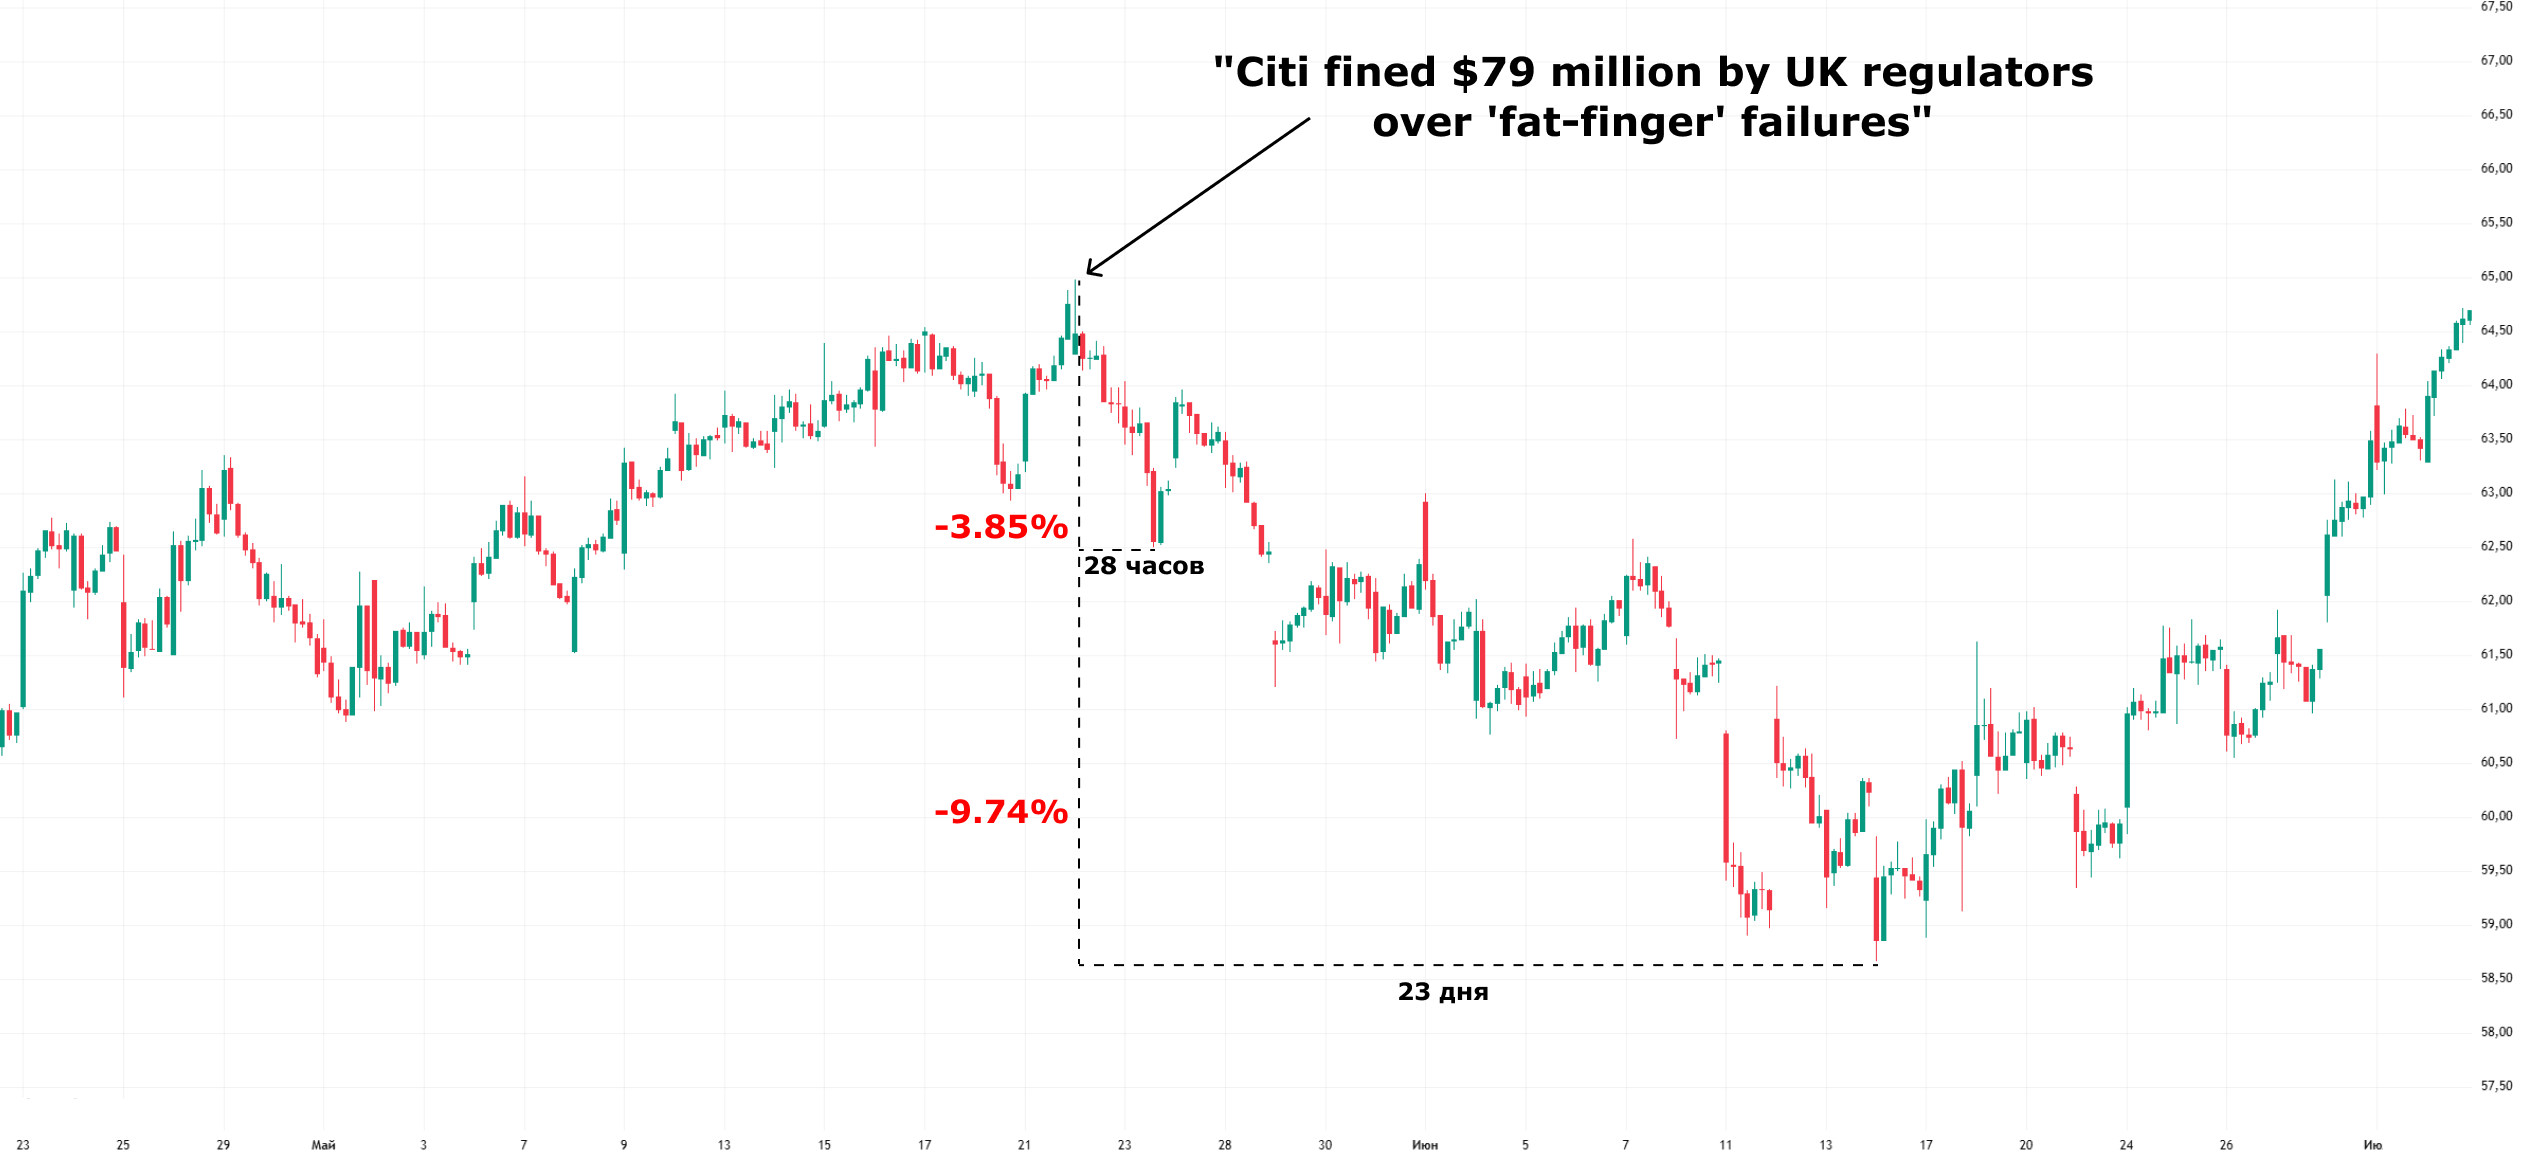
\includegraphics[width=1\linewidth]{img/citi_group.png}
    \caption{Пример падения цены акций одного из крупнейших банков США, Citi Group (C.NYSE),
    из-за обвинений в недостаточном контроле за торговыми операциями, что вызвало падение европейских акций}
    \label{fig:citi_group}
\end{figure}

Сама новостная статья от Reuters послужила сигналом для продажи актива, а на Изображении \ref{fig:citi_group} явно виден
переломный момент с резким падением цены, небольшим откатом и дальнейшей сменой глобального тренда почти на месяц.

Без FinABYSS подобные сигналы часто теряются в потоке новостей, в то время как разработанная система упрощает обнаружение
триггерных событий, посредством реализации возможности отслеживания значимых для конкретного портфеля кластеров.

Второй кейс связан с публикацией от 30 августа 2024 года о возможном отзыве лицензии и штрафе AU\$ 67 млн в отношении крупнейше
 австралийской компании по азартным играм --- The Star Entertainment Group LTD (рис. \ref{fig:star_entertainment}). Новость сообщала
 об обвинениях  в отмывании денег. Акции оказались заморожены на месяц, а при возобновлении торгов их стоимость рухнула на 55\%.

\begin{figure}[H]
    \centering
    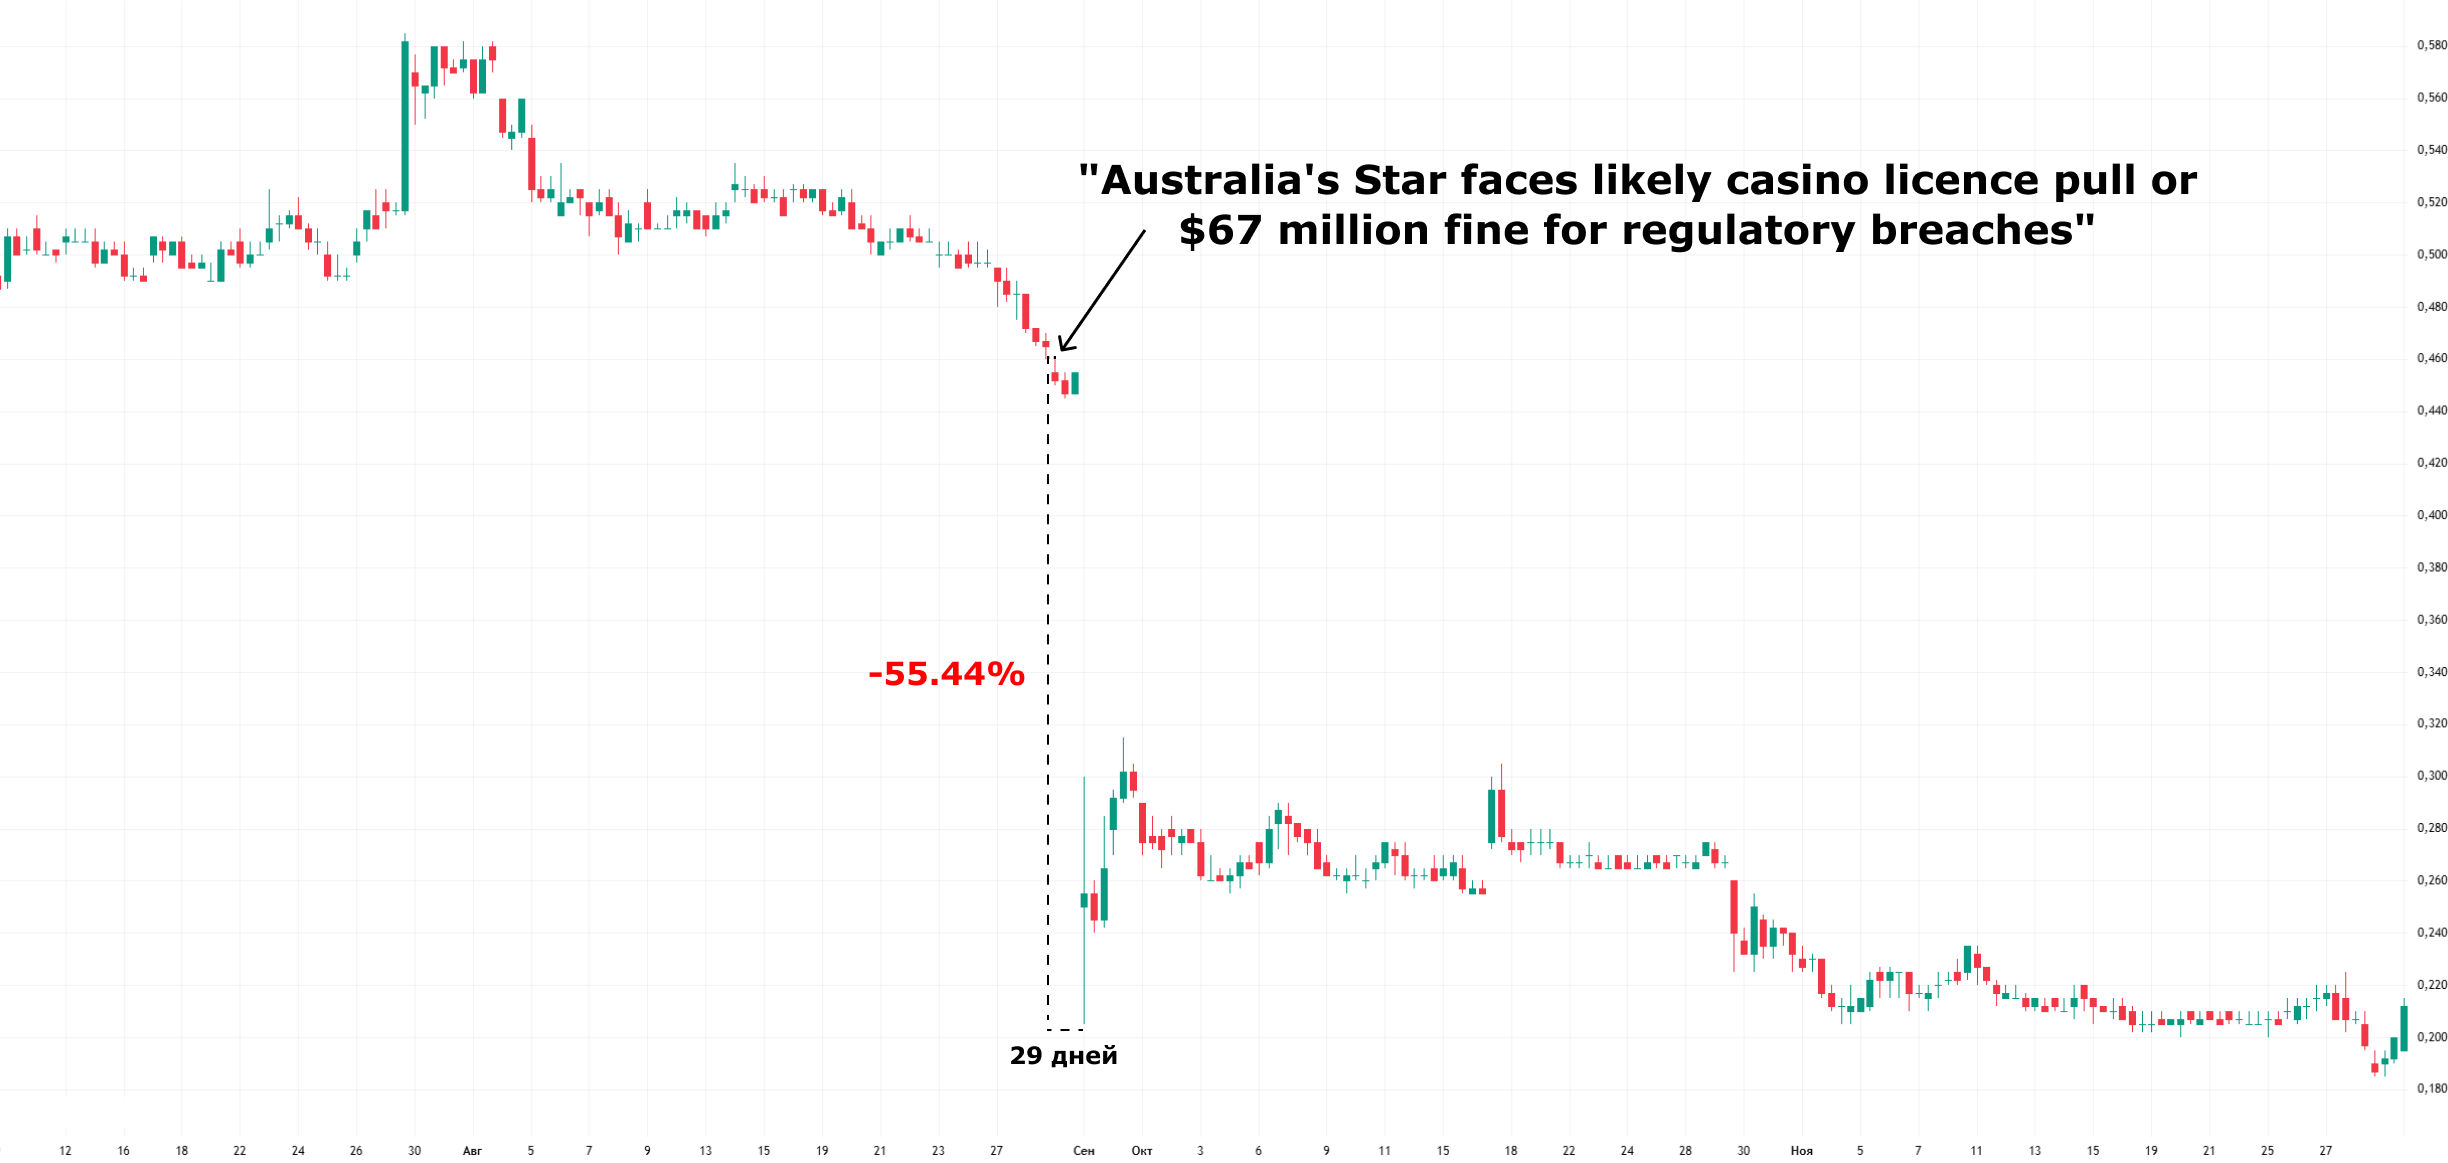
\includegraphics[width=1\linewidth]{img/star_entertainment.png}
    \caption{Пример того, как акции австралийской компании Star Entertainment Group LTD (SGR.ASX)
    обвалились и торговля ими была временно приостановлена из-за судебного разбирательства по отмыванию денег.}
    \label{fig:star_entertainment}
\end{figure}

Важно отметить, что торговля была приостановлена через сутки после публикации новости, что хоть
и является достаточным интервалом для обнаружения сигнала о продаже. Однако для рядового не вовлеченного
во внутридневную торговлю инвестора, данный сигнал весьма вероятно был бы незаметен, что привело бы
к ужасающей ситуации, когда инвестор не может продать обесценившийся актив и вынужден держать очевидный
убыток неопределенно длительный срок.

В обоих случаях, имея систему FinABYSS финансовый аналитик или инвестор мог бы одним из первых узнать
о данных инцидентах и незамедлительно отреагировать на рыночные сигналы. Простейшим способом своевременно
узнавать о триггерах является модуль активо-ориентированного отслеживания, который позволяет задать фильтры
по конкретному тикеру, источнику и тематике, чтобы получать только таргетированные сигналы.

В перспективе, после полной реализации и обучения архитектуры, предложенной в \hyperref[sec:architecture]{Разделе 3.1}, станет возможным
настройка фильтрации новостей по их сентименту, а также настройка пользовательского порога для обнаружения
значимо позитивных или негативных новостей.

Таким образом, FinABYSS выводит финансовую аналитику на совершенно новый уровень: вместо бессистемного
мониторинга СМИ и статей он получает готовые к действию алерты, визуализацию и прогнозную поддержку.
Семантическая карта уже сегодня становится неотъемлемой частью рабочего процесса, а по мере расширения
модальностей и внедрения предиктивного механизма её ценность будет лишь расти.


It is important to note that trading was halted 24 hours after the news was published, which is a sufficient
interval for a sell signal to be detected. However, for the average investor not involved in intraday trading,
this signal would very likely have been undetectable, leading to the dire situation of an investor unable to sell
a depreciating asset and forced to hold an obvious loss indefinitely.

In both cases, with FinABYSS, a financial analyst or investor would be among the first to recognize these incidents
and react immediately to market signals. The simplest way to learn about triggers in a timely manner is the asset-based
tracking module, which allows you to set filters by specific ticker, source, and topic to receive only targeted signals.

Eventually, once the architecture proposed in \hyperref[sec:architecture]{Section 3.1} is fully implemented and trained, it will be possible
to customize the filtering of news by its sentiment, as well as setting a custom threshold to detect meaningfully
positive or negative news.

FinABYSS thus takes financial analytics to a whole new level: instead of haphazard monitoring of media and articles,
it gets ready-to-action alerts, visualization, and predictive support. The semantic map is already becoming an integral
part of the workflow, and its value will only grow with the expansion of modalities and the introduction of a predictive
mechanism.

\subsection{Semantic De-duplication Solution}
\subsubsection{Mathematical Formulaion}
\sloppy  % Helps to alleviate overfull hbox warnings

Within the framework of this study, a novel deduplication approach was developed based on the analysis of the semantic content of objects.
Although in the present work the entity is a text, the method can be readily generalized to any objects that admit a vector representation
in a semantic space.

Each article is represented as a sequence of embeddings:

\begin{equation}
    x_i \subset \mathbb{R}^{t\times d}
\end{equation}

where $t$ is the number of tokens and $d$ is the dimensionality of the semantic vector space. For subsequent analysis, instead of the raw set of embeddings,
their convex hull is used, denoted as $\operatorname{CH}(x_i)$ or, for brevity, $\operatorname{CH}_i$. The uniqueness of a text is quantified by the volume
of this convex hull, $\mathrm{vol}(\operatorname{CH}_i)$.

\textbf{Accounting for the Intersections of Convex Hulls.} Direct subtraction of the intersections between $\operatorname{CH}_i$ and the hulls of other
texts may lead to multiple counting. To eliminate this issue, the inclusion--exclusion principle is applied.

Let the set of all articles except $i$ be denoted by

\begin{equation}
    \mathbb{I} = \{1, \ldots, N\} \setminus \{i\}.
\end{equation}

The intersection of $\operatorname{CH}_i$ with the hulls of articles indexed by subsets $\mathbb{J} \subseteq \mathbb{I}$ is expressed as:

\begin{equation}
    \mathrm{vol}\Big(\operatorname{CH}_i \cap \bigcap_{j \in \mathbb{J}}\operatorname{CH}_j\Big).
\end{equation}

Then, the volume of the intersection of $\operatorname{CH}_i$ with the union of the hulls of the remaining articles is computed as:

\begin{equation}\label{eq:inclusion-exclusion_substituting}
    \mathrm{vol}\left(\operatorname{CH}_i \cap \bigcup_{j \in \mathbb{I}}\operatorname{CH}_j\right)
    =
    \sum_{k=1}^{N-1} (-1)^{k-1} \sum_{\substack{\mathbb{J} \subseteq \mathbb{I} \\ |\mathbb{J}| = k}}
    \mathrm{vol}\left(\operatorname{CH}_i \cap \bigcap_{j \in \mathbb{J}}\operatorname{CH}_j\right).
\end{equation}

The uniqueness of article $i$ is defined as the fraction of its convex hull’s volume that is not occupied by intersections with the hulls of other articles:

\begin{equation}
    \mu_i = \frac{\mathrm{vol}\Big( \operatorname{CH}_i \setminus \bigcup_{j \in \mathbb{I}} \operatorname{CH}_j\Big)}{\mathrm{vol}\Big( \operatorname{CH}_i\Big)}.
\end{equation}

By decomposing $\operatorname{CH}_i$ into the intersection region and its complement, we obtain:

\begin{equation}
    \mu_i = 1 - \frac{\mathrm{vol}\left(\operatorname{CH}_i \cap \bigcup_{j \in \mathbb{I}}\operatorname{CH}_j\right)}{\mathrm{vol}\left(\operatorname{CH}_i\right)}.
\end{equation}

Substituting the inclusion--exclusion formulation \ref{eq:inclusion-exclusion_substituting}, the final expression becomes:

\begin{equation}\label{eq:uniqueness}
    \mu_i = 1 - \frac{1}{\mathrm{vol}\big(\operatorname{CH}_i\big)}
    \sum_{k=1}^{N-1} (-1)^{k-1} \sum_{\substack{\mathbb{J} \subseteq \mathbb{I} \\ |\mathbb{J}| = k}}
    \mathrm{vol}\Big(\operatorname{CH}_i \cap \bigcap_{j \in \mathbb{J}}\operatorname{CH}_j\Big).
\end{equation}

The value $\mu_i \in [0, 1]$ characterizes the text's uniqueness: $\mu_i = 1$ indicates no intersections with other texts (complete uniqueness),
while $\mu_i = 0$ implies that the semantic volume of the text is entirely occupied by intersections with the hulls of other texts.

\subsubsection{Pros and Cons}
The proposed method is founded on a theoretically sound representation of text: each article is treated as the convex hull of its token embeddings.
This representation enables a precise definition of an object’s semantic content, facilitates the application of the inclusion–exclusion principle
(inherited from set theory) for accurate calculation of intersection volumes, and normalizes the result so that the final uniqueness measure
lies within the interval $[0,1]$.

In addition to its theoretical rigor, the method offers several advantages:
\begin{itemize}
    \item The use of embeddings for each token allows for capturing subtle distinctions in semantic content, while aggregation via the convex hull
    yields a generalized representation of the text. This approach enables the comparison of texts of varying lengths and topics within a unified vector space.
    \item Normalization of the metric to a $[0,1]$ interval simplifies interpretation.
\end{itemize}

Conversely, the method has several notable drawbacks:
\begin{itemize}
    \item In high-dimensional spaces (e.g., 768 dimensions), the convex hull may become excessively "stretched," resulting in uninformative volume measurements,
    and its geometry may fail to accurately reflect the complex distribution of embeddings.
    \item Embeddings typically possess a complex, often non-linear structure. As the convex hull is the minimal convex set containing the data, it may enclose
    extreme points, leading to an overestimation of the occupied space and, consequently, to skewed evaluations.
    \item Since embeddings can include random noise or artifacts, the convex hull is sensitive to outliers. Minor inaccuracies in embeddings may
    disproportionately enlarge the convex hull’s volume, thus distorting the uniqueness assessment.
    \item Constructing the convex hull and computing volumes in high-dimensional spaces is computationally intensive. Moreover, applying the inclusion–exclusion
    principle to accurately compute intersections between the hulls of texts further complicates calculations, particularly with a large number of documents.
\end{itemize}

These challenges can critically affect the practical application of the method; however, some can be mitigated through engineering solutions.

The sensitivity to noise (item 3) can be partially alleviated by using the [CLS] token as the centroid of the convex hull. Introducing a coefficient
$\delta$ to normalize the "concavity" of the hull in the direction of the [CLS] embedding helps to diminish the impact of noisy components.

The computational burden (item 4) can be addressed through various strategies:
\begin{itemize}
    \item Regulating the number of inclusion–exclusion pairs (the hyperparameter $N$ in the summation) allows for an approximate evaluation
    of uniqueness while reducing computational demands.
    \item Employing dimensionality reduction algorithms, such as UMAP, t-SNE, or PCA, can project the original space onto a lower-dimensional one,
    substantially decreasing computational costs, though potentially at the expense of some accuracy.
    \item Approximating the volume using Monte Carlo methods offers an alternative that lessens computational load.
\end{itemize}

The method of representing semantic uniqueness of text via the convex hulls of embeddings boasts several theoretical advantages (robust normalization,
applicability of the inclusion–exclusion principle, and consistent interpretability of the result). Nevertheless, its practical deployment necessitates
addressing challenges related to high dimensionality, non-linear distributions of embeddings, and substantial computational costs. Future research may
focus on developing more robust and computationally efficient methods for assessing text uniqueness while accommodating these limitations.


    \newpage
    \specialsection{Заключение}
    \label{sec:conclusion}
    \textbf{Disparity in Access to Financial Resources.} During the study, it was found that there exists a significant barrier for individual
researchers who lack the financial resources required for expensive data collection, infrastructure rental, and the time needed to develop
a system entirely from scratch.

The financial community — which includes news outlets, data aggregators, professional traders, and investment funds — often does not facilitate
the development of publicly available tools for extracting value from financial instruments. On the contrary, several market participants deliberately
create additional obstacles to free data access, while failing to utilize existing resources efficiently. Examples include:

\begin{itemize}
    \item \textbf{Infrastructure limitations.} Restrictions imposed by aggregators and news services (e.g., Yahoo! Finance) impede large-scale data collection.
    \item \textbf{Closed APIs and high tariffs.} Services such as Google Finance and Yahoo! Finance, along with platforms like Twitter and Seeking Alpha,
    offer limited functionality or charge high fees for access.
    \item \textbf{Restrictions on access to analytical tools.} Cases such as BloombergGPT illustrate the deliberate concealment of general-purpose tools.
    \item \textbf{Strict copyright policies.} Tighter copyright conditions result in restricted access to various datasets \parencite{wu2023BloombrgGpt}.
\end{itemize}

Thus, it can be concluded that the financial community contributes to a scarcity of open informational resources by artificially raising
the barriers to access with the aim of reducing competition and limiting the number of independent market players.

This issue is not new --- it has been repeatedly highlighted in several studies (including by the creators of FinBERT \parencite{Yang2020FinBERT});
however, over the past five years the situation has remained virtually unchanged. A crisis also persists in the open-source segment of financial tools.

Despite the widespread restrictive practices, there are proactive participants in the financial sector who strive to distribute information
more equitably. For instance, the financial data provider Alpha Vantage\footnote{URL: \url{https://www.alphavantage.co/}} offers a free and open API
that grants access to a vast array of valuable data, including intraday OHLCV. Although Reddit\footnote{URL: \url{https://www.reddit.com/}} is less
popular than platform X (ex-Twitter)\footnote{URL: \url{https://x.com/}} in the financial community, it also provides an open API and can serve
as an alternative channel for publishing announcements, opinions, and insider information.

In addition, aggregators such as FinURLs\footnote{URL: \url{https://finurls.com/}} and MarketWatch\footnote{URL: \url{https://www.marketwatch.com/}}
represent important information sources. FinURLs compiles links to historical news from 24 sources over several years. Despite the lack
of a dedicated API and certain interface inconveniences for data extraction, this resource remains valuable. At the same time,
MarketWatch boasts a more advanced infrastructure by offering not only links to news articles but also quantitative data, as well as the ability
to obtain information on specific markets, assets, or indices.

Individual yet significant sources, such as the websites of certain companies and government agencies, also deserve attention. For example,
the SEC\footnote{URL: \url{https://www.sec.gov/}} provides free access to historical financial reports (e.g., 10-K and 10-Q) via an RSS feed,
thereby promoting more equitable access to information. However, even these open datasets are frequently accompanied by technical challenges:
precise timestamps are often missing or the website structure is disrupted, which complicates automated data extraction.

It should be noted that nearly all real-time data are available without significant restrictions, as most services promptly provide such information.
Nevertheless, the collection of both historical and real-time data regularly encounters ethical and copyright issues, which remain an important aspect
in the practical use of these resources.

In summary, despite various initiatives aimed at expanding access to financial data, the overall landscape is still characterized by artificially
high barriers. These restrictions contribute to a shortage of open tools, which in turn reduces market competition and limits opportunities
for independent researchers. Therefore, the development of methodologies aimed at the free and equitable dissemination of information remains
an urgent task, requiring a comprehensive approach that takes technical, ethical, and legal aspects into account.

    \newrefcontext[sorting=ntvy]
    \printbibliography[env=gostbibliography, title=Источники литературы]
\end{document}